\documentclass{article}

\usepackage[margin=2.5cm,left=2cm,includefoot]{geometry}
\usepackage{graphicx}
\usepackage{float}
\usepackage[space]{grffile}
\usepackage{hyperref}
\usepackage[export]{adjustbox}
\usepackage{multicol}
\usepackage{caption}
\usepackage{hyperref}
\usepackage{listings}
\usepackage{vhistory}
\usepackage{titlesec}

\setcounter{secnumdepth}{4}

\titleformat{\paragraph}
{\normalfont\normalsize\bfseries}{\theparagraph}{1em}{}
\titlespacing*{\paragraph}
{0pt}{3.25ex plus 1ex minus .2ex}{1.5ex plus .2ex}

% Header and footer
\usepackage{fancyhdr}
\pagestyle{fancy}

\rhead{COS301}
\lhead{User Manual Document}
\fancyfoot[R]{Page \thepage}

\renewcommand{\headrulewidth}{2pt}
\renewcommand{\footrulewidth}{1pt}

\begin{document}

	\begin{titlepage}
		\begin{center}
			
\includegraphics[width=10cm]{images/marketlead_logo.png}  \\
			[0.5cm]
			\huge{
			User Manual Document\\
			}
			
			\line(1,0){300}\\
			[0.2cm]
			\LARGE{Project: MarketLead.io\\
			Client: RetroRabbit} \\
			\line(1,0){300}\\
			\LARGE{Team: Valknut Solutions}\\
			[1.0cm]
			\large{Version: 1.1}\\
			[1.0cm]
			\large
			{
			\begin{itemize}
				\item 13054903 - Charl Jansen van Vuuren
				\item 13044924 - Kevin David Heritage
				\item 13176545 - Quinton Weenink\\
			\end{itemize}
			}
			\textsc{\large}\\
		[3.0cm]
		\textsc{\large  Department of Computer Science}\\
		[0.5cm]
		\textsc{\large \today}\\
		\end{center}
	\end{titlepage}
	
	\cleardoublepage
	% Start of the revision history table
	\begin{versionhistory}
  		\vhEntry{1.0}{27.7.2016}{CJvV,KDH,QW}{in progress}
  		\vhEntry{1.1}{9.9.2016}{CJvV,KDH,QW}{Changed Project name. Updates for new use cases and modules}
  		\vhEntry{1.2}{12.10.2016}{CJvV,KDH,QW}{Update manual according to feedback. Added new use cases. Updated the logo to the product logo.}
	\end{versionhistory}	
	
	\cleardoublepage
	\tableofcontents
	\cleardoublepage
	
	\section{General Information}
		\subsection{System Overview}
			MarketLead.io is a real time marketing and lead gathering application with multiple integration points from social media and other formats.\\
			A business can manage and respond to leads and analyze their current customers. We expose and link companies to their future customers in an easy and pluggable manner.\\
			This document contains information related to the use of the MarketLead.io system and how to use it. The purpose of the system is to gather information from various social media platforms (i.e. Facebook Messenger, Facebook Lead Ads and We chat).
			The data that was gathered can then be visualized in different graphs for analysts to view and gain insights from all of the integration points. Customers do not necessarily interact with our system directly but they can by completing the static lead form. \ref{fig:lead}
			A marketer can register their different social media platforms to interact with the system through the website.
			The following documentation is a guide on how to interact and use the web interface for marketers, analysts and administrators and in one case the future customer.
			Working through this user manual can give anyone interacting with the web interface more information on how to use the system efficiently and correctly.

		\subsection{System Configuration}
			The main input of data to the system will be from the various social media platforms.
			Marketers and analysts will interact with the system by the use of the web interface.
			\begin{figure}[H]
				\includegraphics[width=\textwidth]{images/user_server1.png}
				\caption{System overview}
				\label{fig:sysOverview}
			\end{figure}

			\begin{figure}[H]
				\includegraphics[width=\textwidth]{images/analyst_server.png}
				\caption{Stakeholders}
				\label{fig:stakeholders}
			\end{figure}

		\subsection{Installation}
			The system does not have to be installed, however an up to date web browser is required to view the web site that interacts with the system. Mozilla Firefox or Google Chrome is recommended.

	\section{Getting Started}
		A user/client needs to be signed up for the various social media platforms that the system uses (Facebook, WeChat).
		Marketers should also have accounts with the various social media platforms in order to add hooks to the adverts and messenger accounts to interact with the system.
		Analysts will receive a login from an administrator of the system to be able to log into the system and see analytics.\\
		Marketers and analysts can open their web browser (Mozilla Firefox/Google Chrome recommended) and navigate to \href{https://marketlead.herokuapp.com}{MarketLead.io} to get started with the various tasks.
		When the marketer/analyst is done using the system they can simple close the web browser window/tab to end their session with the system.

	\section{Using the system}
		Note: All screen shots were taken while using the Google Chrome browser.
		\subsection{Home}
			\begin{figure}[H]
				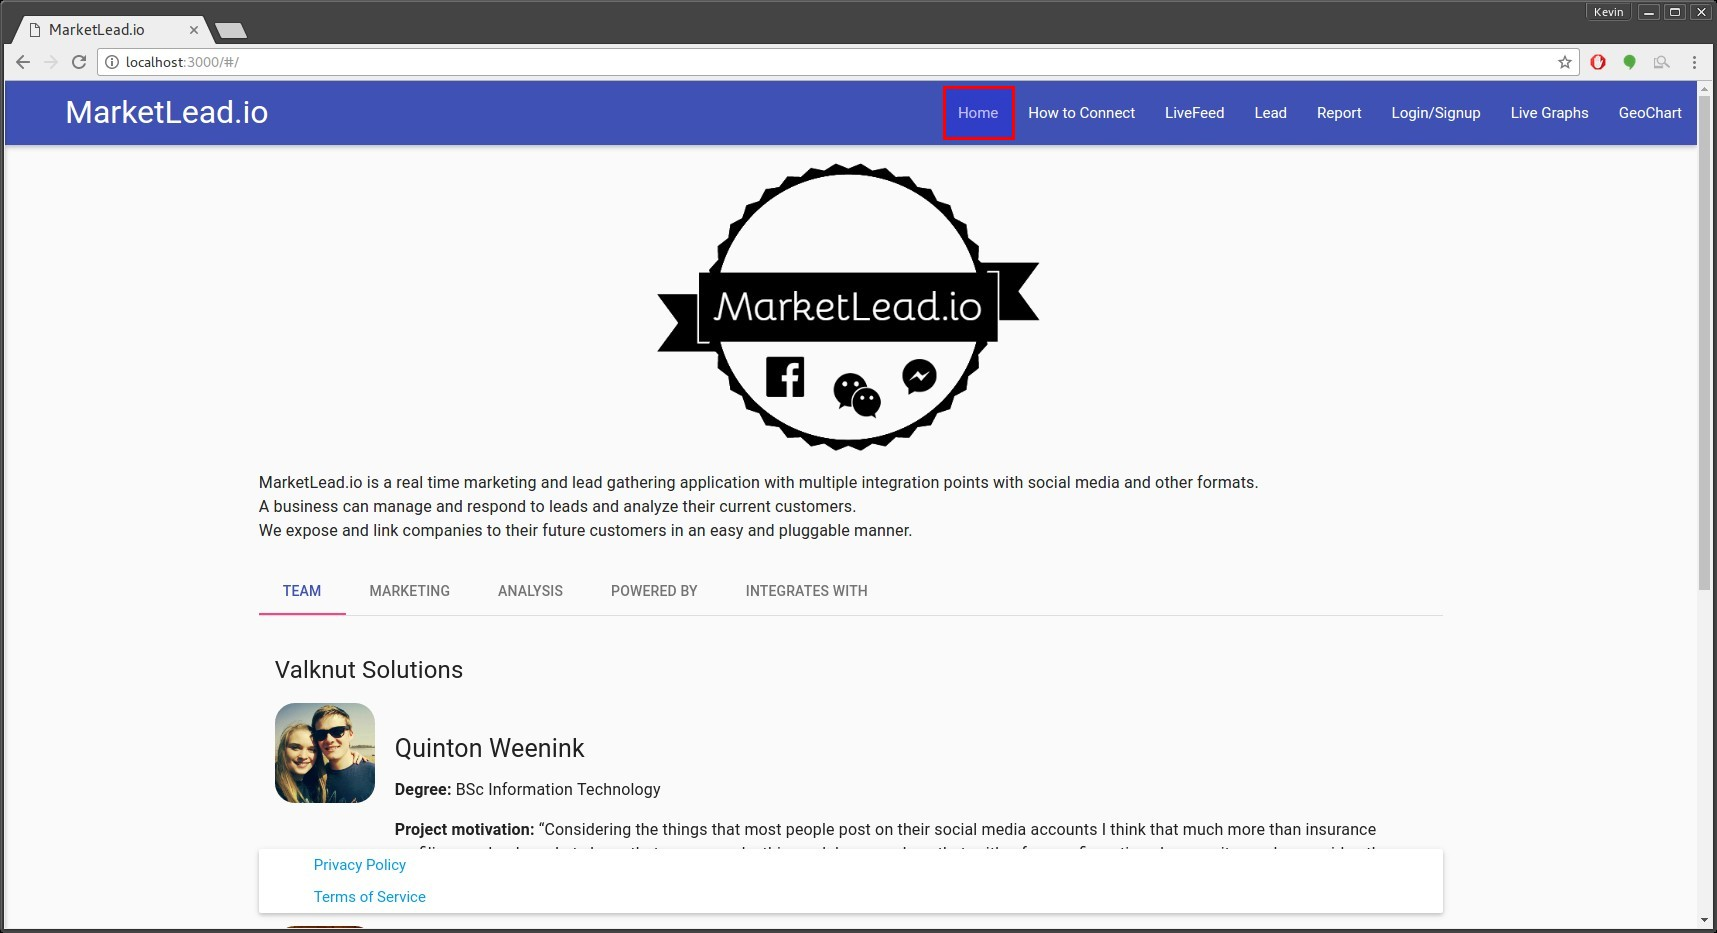
\includegraphics[width=\textwidth]{images/home.jpg}
				\caption{Home page}
				\label{fig:home}
			\end{figure}

			\begin{itemize}
				\item This page will be loaded when first visiting the web page.
				\item General information about the system can be found here.
			\end{itemize}

			\subsubsection{Team}
				\begin{figure}[H]
					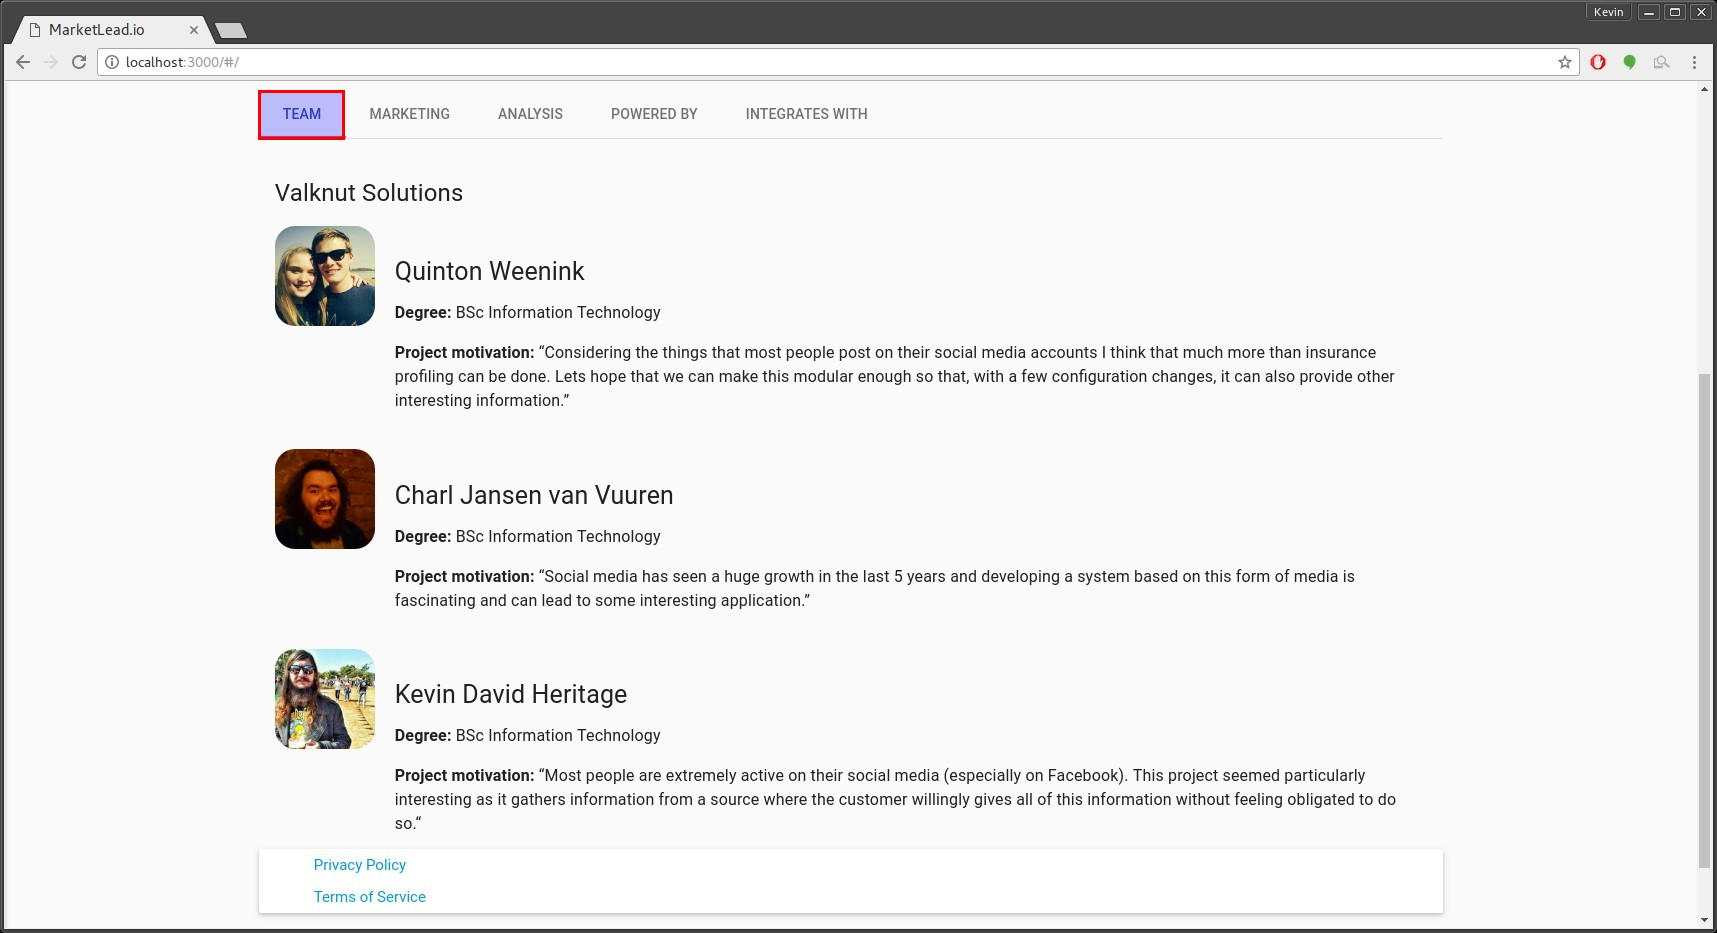
\includegraphics[width=\textwidth]{images/home_team.jpg}
					\caption{Home Page - Team}
					\label{fig:homeTeam}
				\end{figure}

				\begin{itemize}
					\item On this page you can find information on the team that developed the platform.
				\end{itemize}

			\subsection{Marketing}
				\begin{figure}[H]
					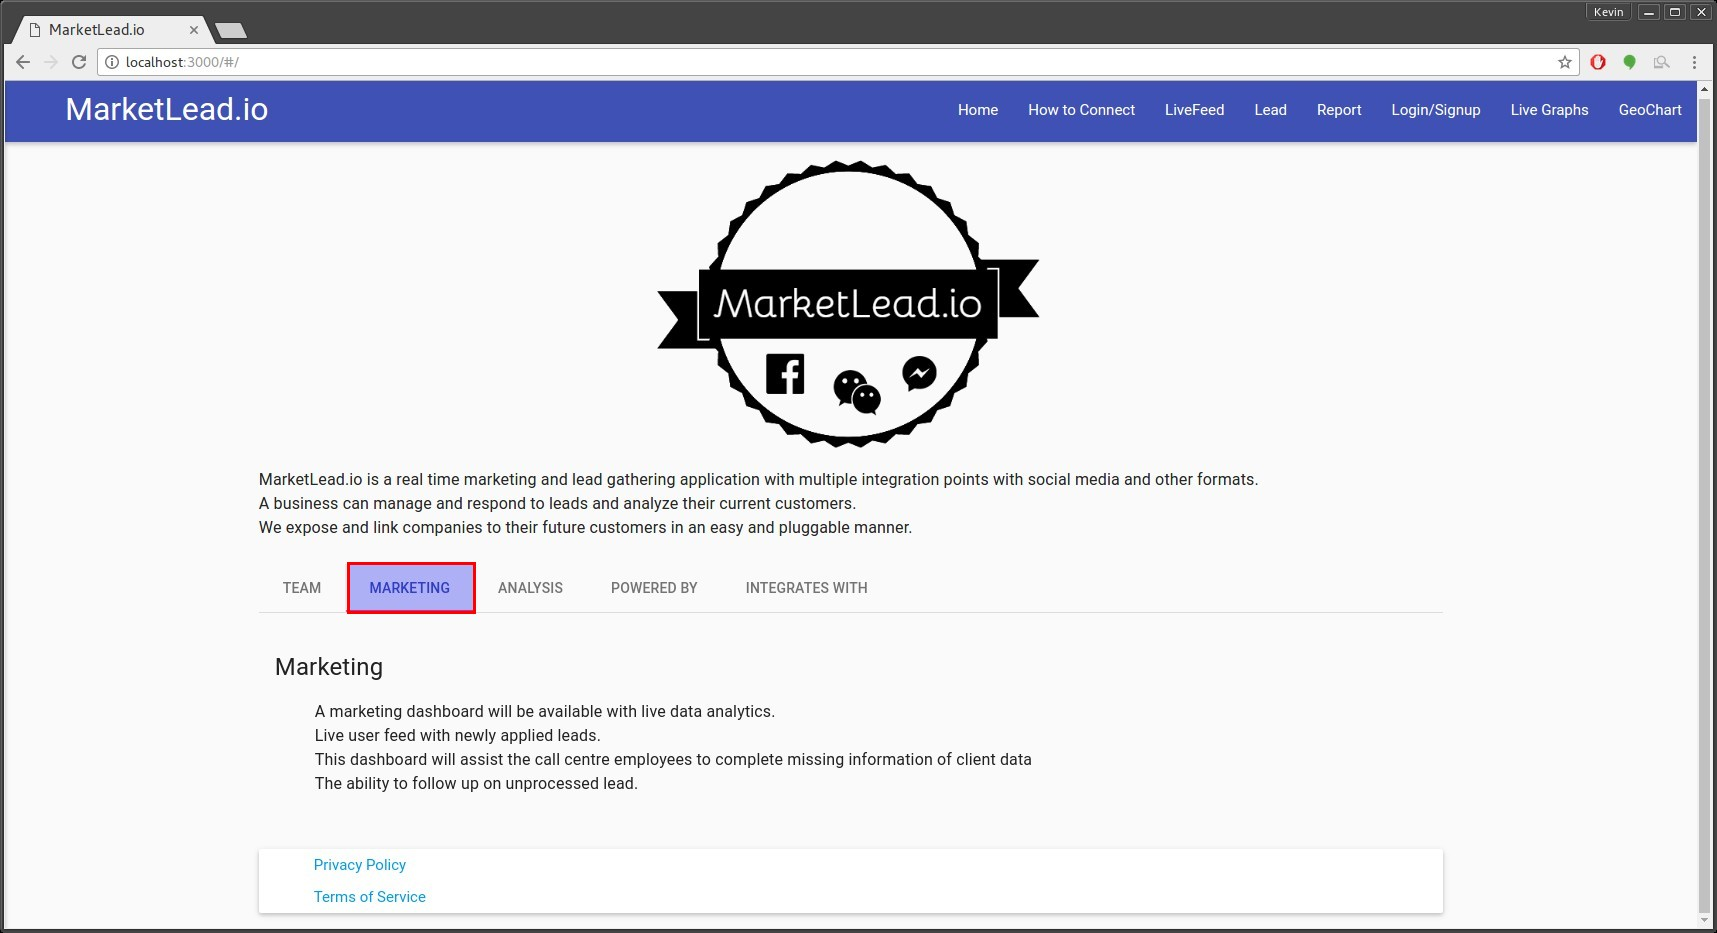
\includegraphics[width=\textwidth]{images/home_marketing.jpg}
					\caption{Home Page - Marketing}
					\label{fig:homeMarketing}
				\end{figure}

			\subsubsection{Analysis}
				\begin{figure}[H]
					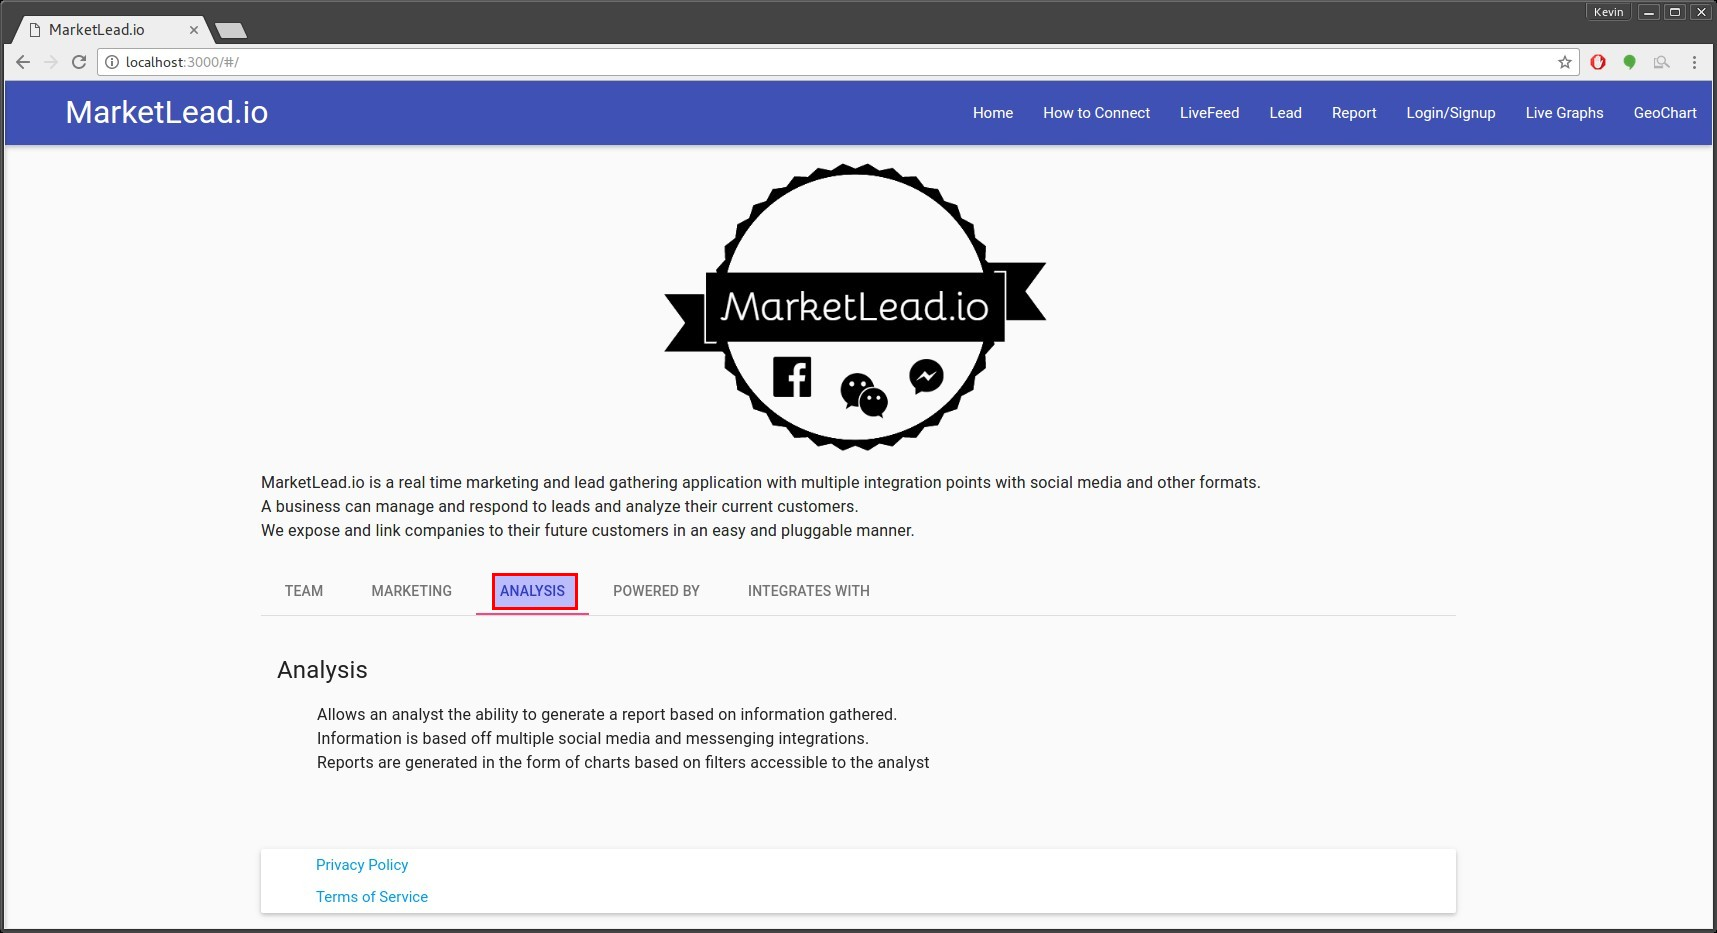
\includegraphics[width=\textwidth]{images/home_analysis.jpg}
					\caption{Home Page - Analysis}
					\label{fig:homeAnalysis}
				\end{figure}

			\subsubsection{Powered By}
				\begin{figure}[H]
					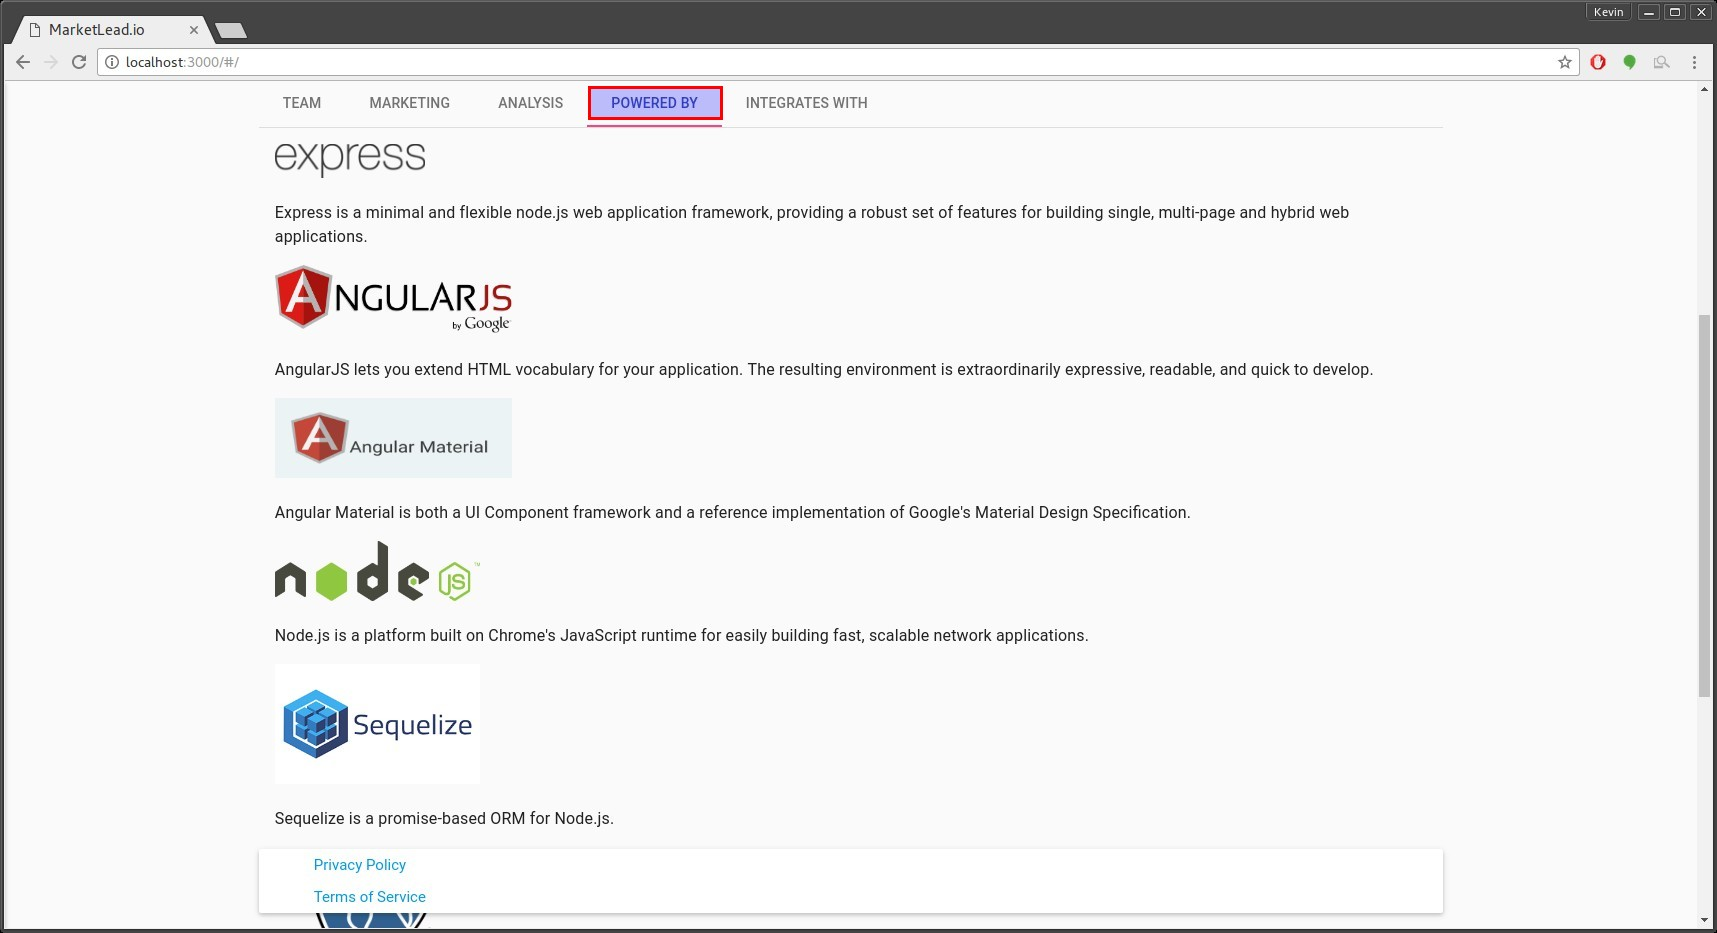
\includegraphics[width=\textwidth]{images/home_powered_by.jpg}
					\caption{Home Page - Powered By}
					\label{fig:homePoweredBy}
				\end{figure}

				\begin{itemize}
					\item Shows the technologies that were used to create the system.
				\end{itemize}

			\subsubsection{Integrates With}
				\begin{figure}[H]
					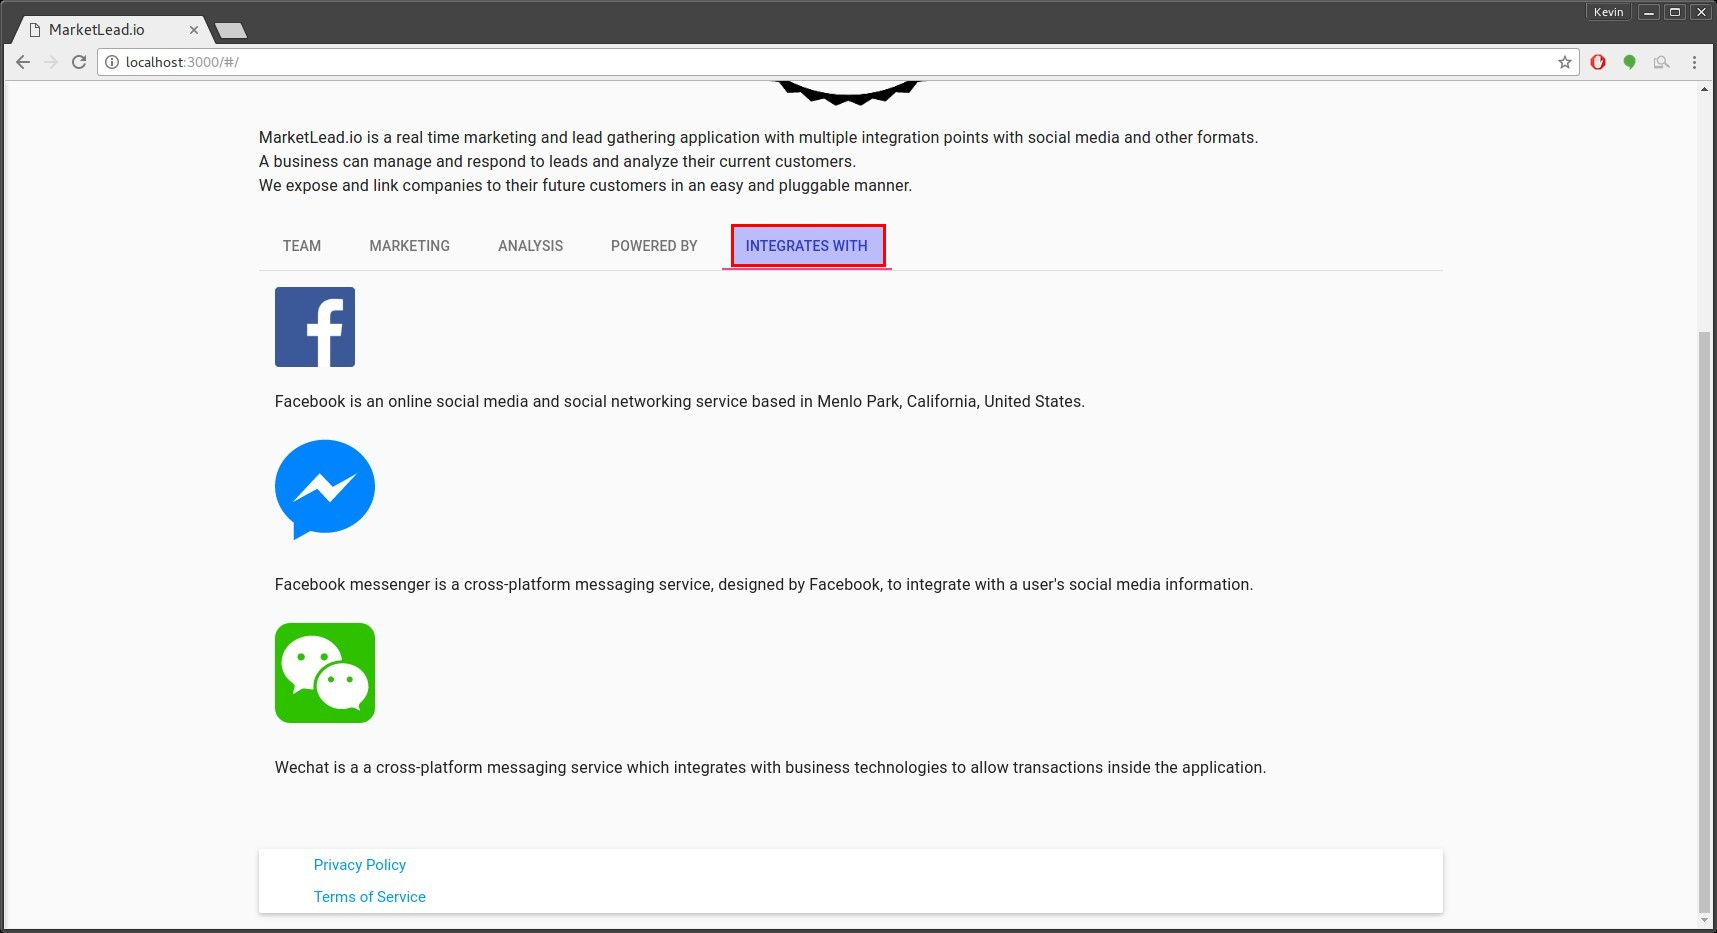
\includegraphics[width=\textwidth]{images/home_integrates_with.jpg}
					\caption{Home Page - Integrates With}
					\label{fig:homeIntegratesWith}
				\end{figure}

				\begin{itemize}
					\item Social media platforms that are currently supported by the system.
				\end{itemize}

		\subsection{How to Connect}
			\begin{figure}[H]
				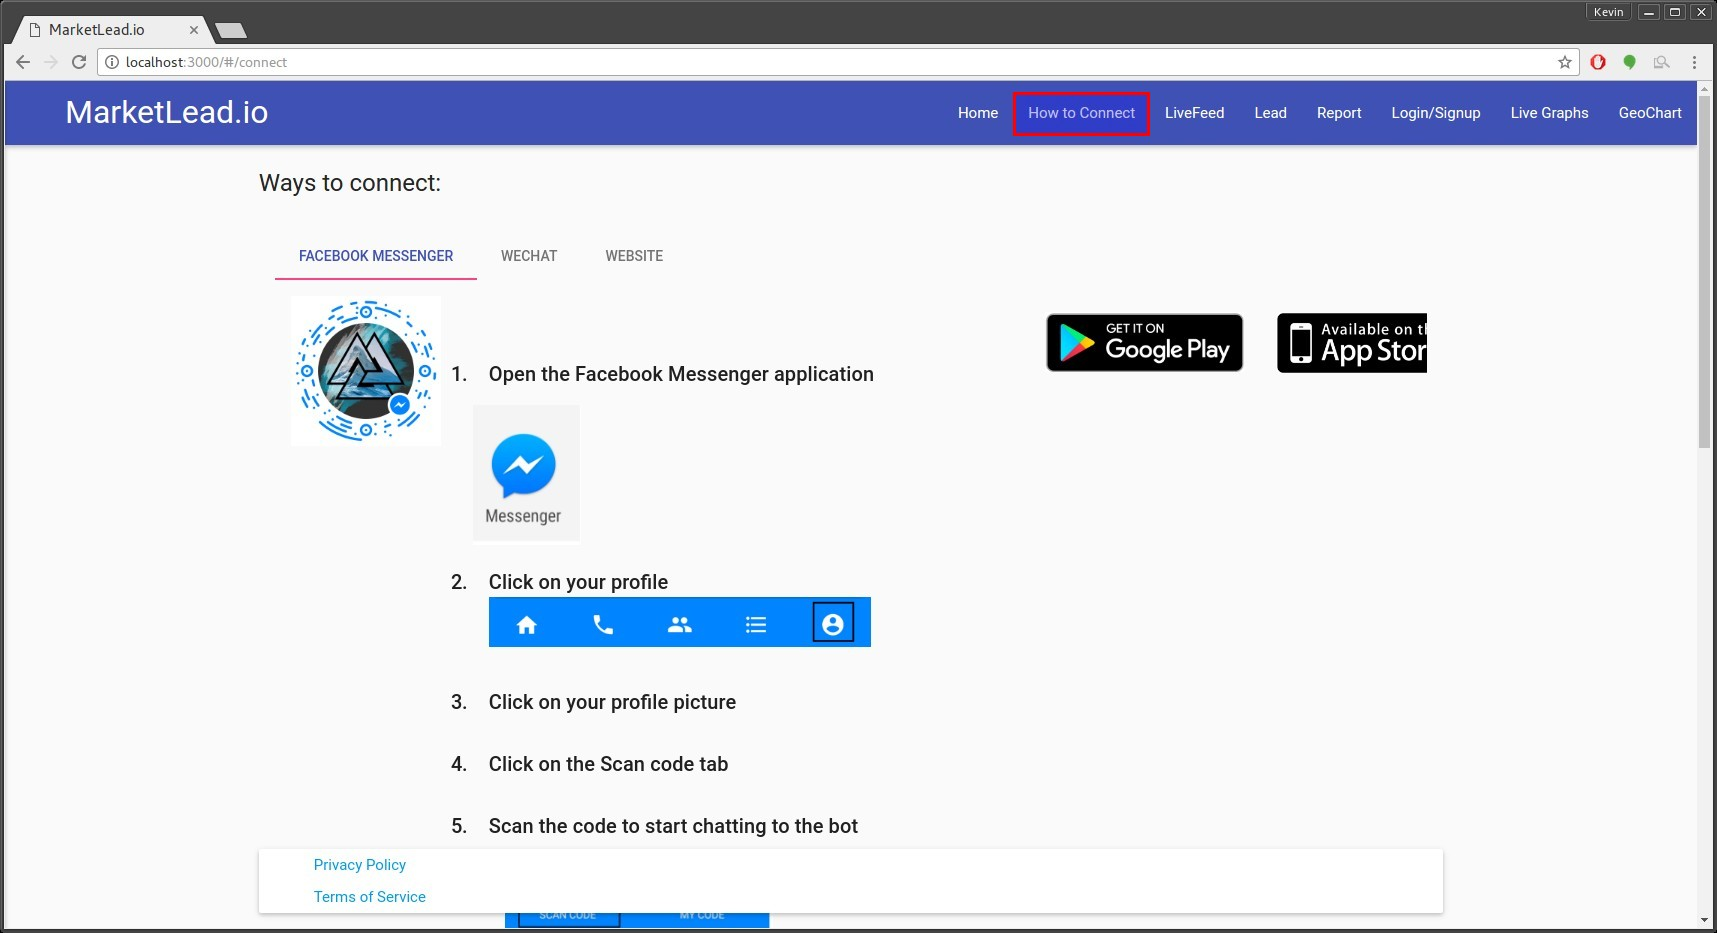
\includegraphics[width=\textwidth]{images/how_to_connect.jpg}
				\caption{How to Connect}
				\label{fig:howToConnect}
			\end{figure}

			\begin{itemize}
				\item This page gives users a guide on how they can interact with the system through the various social media platforms.
			\end{itemize}

			\subsubsection{Facebook Messenger}
				\begin{figure}[H]
					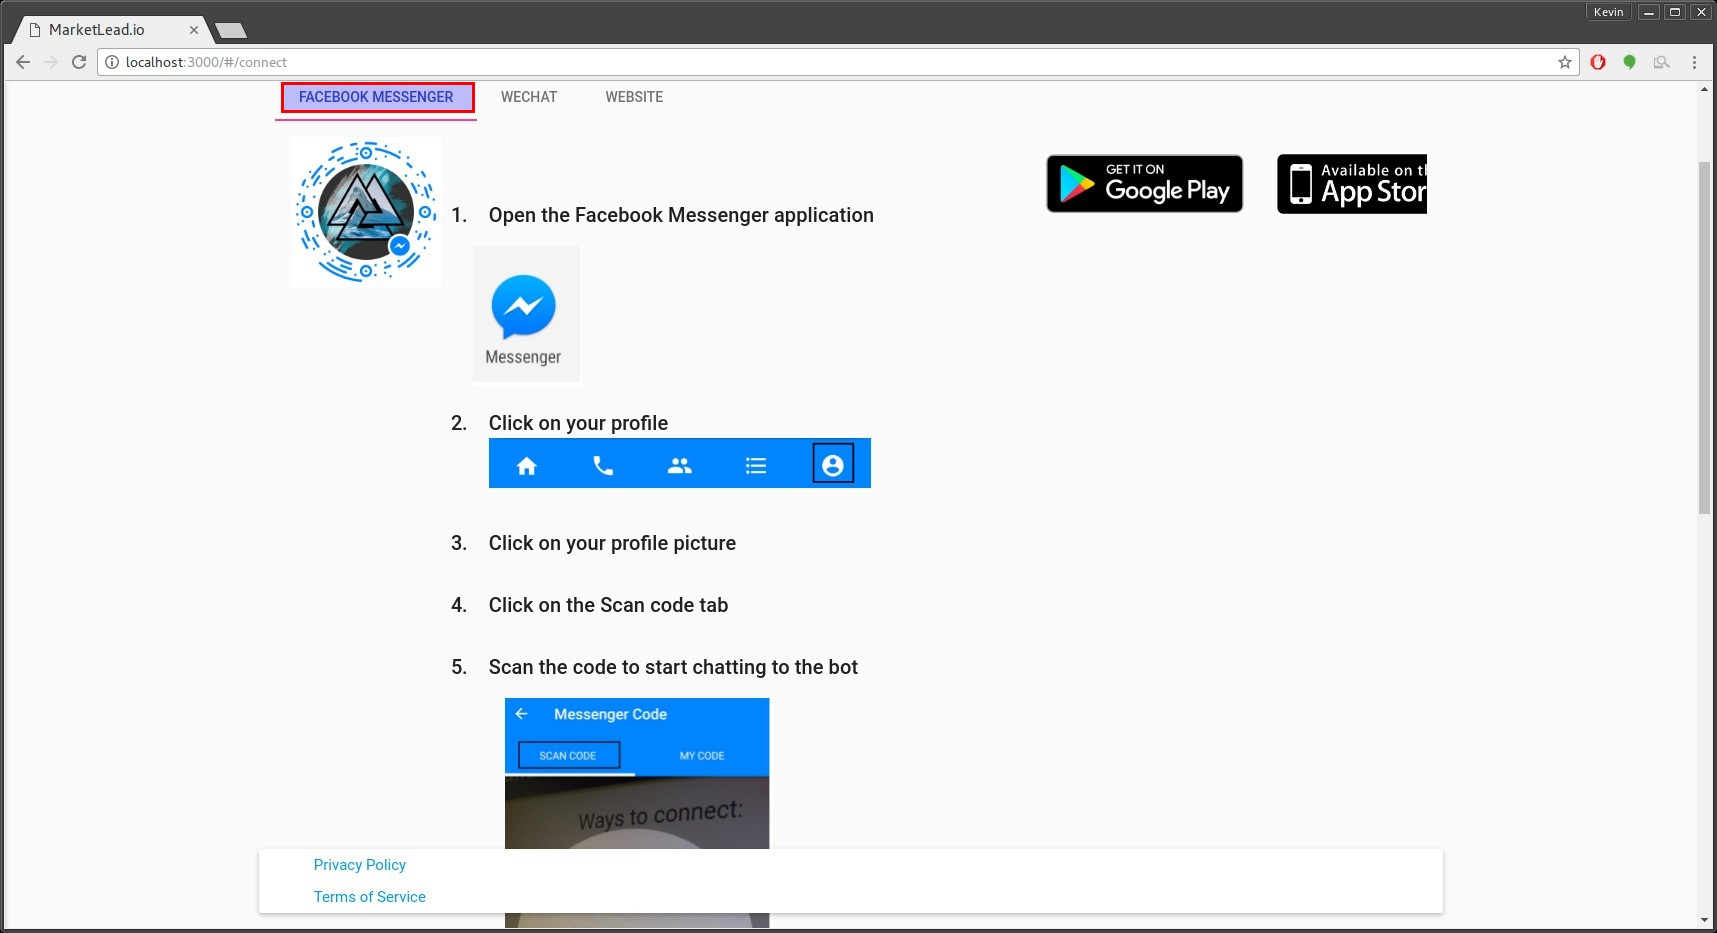
\includegraphics[width=\textwidth]{images/how_to_connect_facebook_messenger.jpg}
					\caption{How to Connect - Facebook Messenger}
					\label{fig:howToConnectFacebookMessenger}
				\end{figure}

				\begin{itemize}
					\item Gives the client a guide on how to connect with our Facebook Messenger bot.
					\item There are also links for downloading the Facebook Messenger application for Android and iOS on this page.
				\end{itemize}

			\subsubsection{WeChat}
				\begin{figure}[H]
					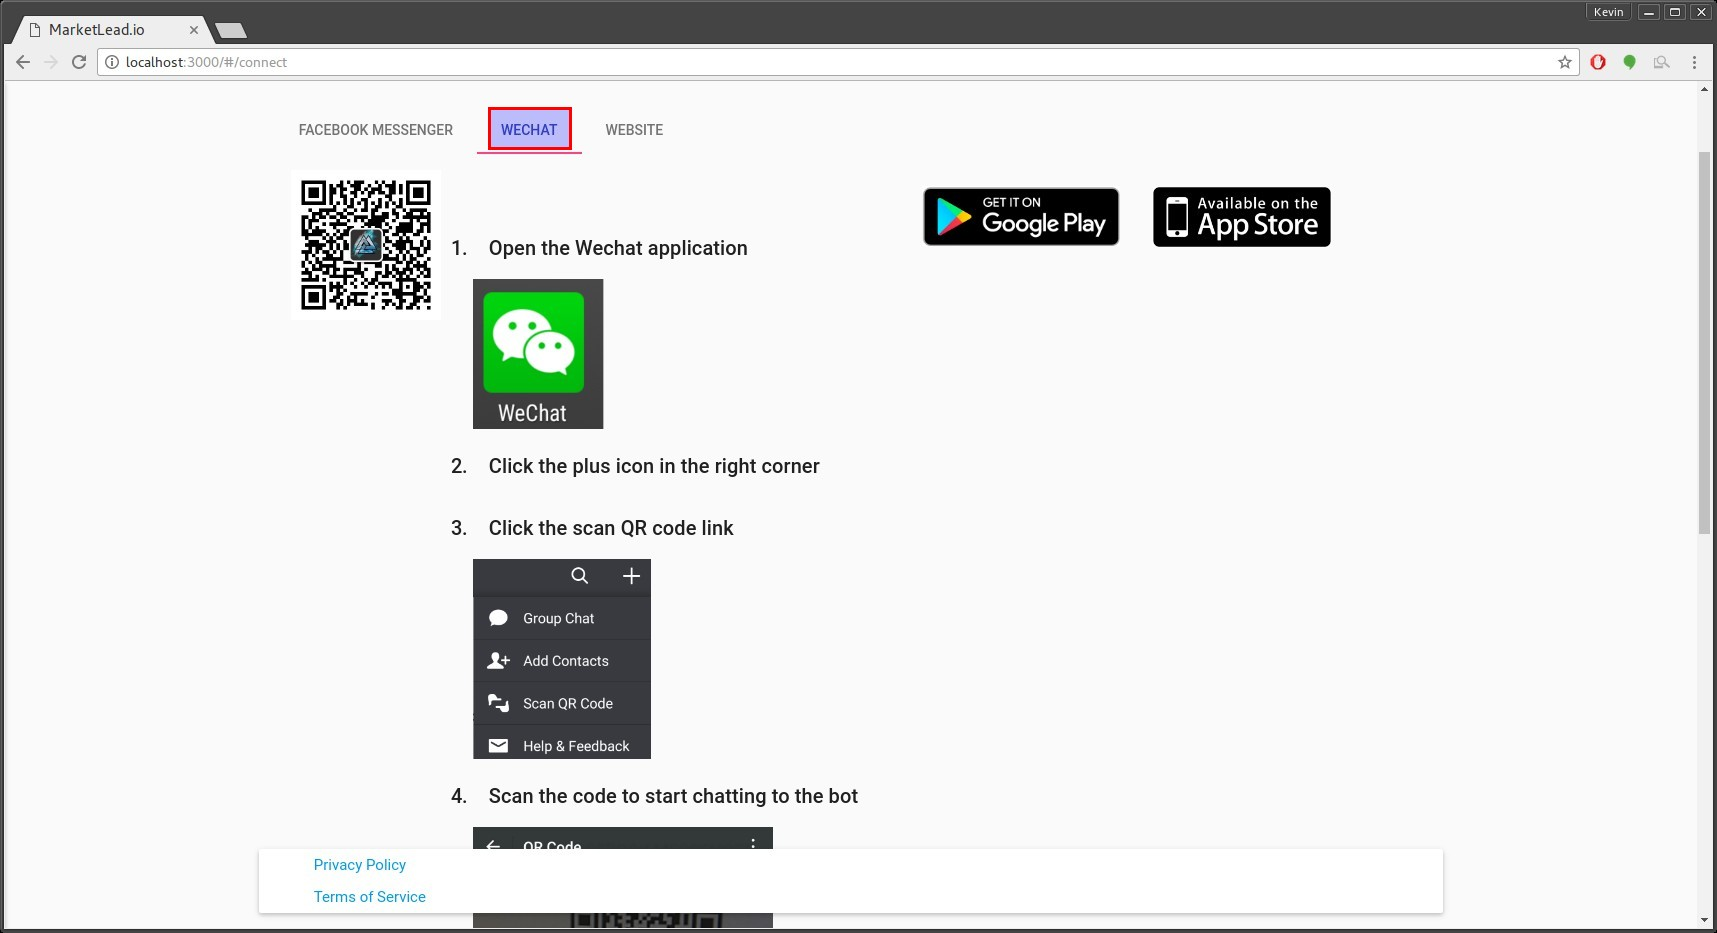
\includegraphics[width=\textwidth]{images/how_to_connect_wechat.jpg}
					\caption{How to Connect - WeChat}
					\label{fig:howToConnectWeChat}
				\end{figure}

				\begin{itemize}
					\item Gives the client a guide on how to connect with our WeChat messenger bot.
					\item There are also links for downloading the WeChat messenger application for Android and iOS on this page.
				\end{itemize}

			\subsubsection{Website}
				\begin{figure}[H]
					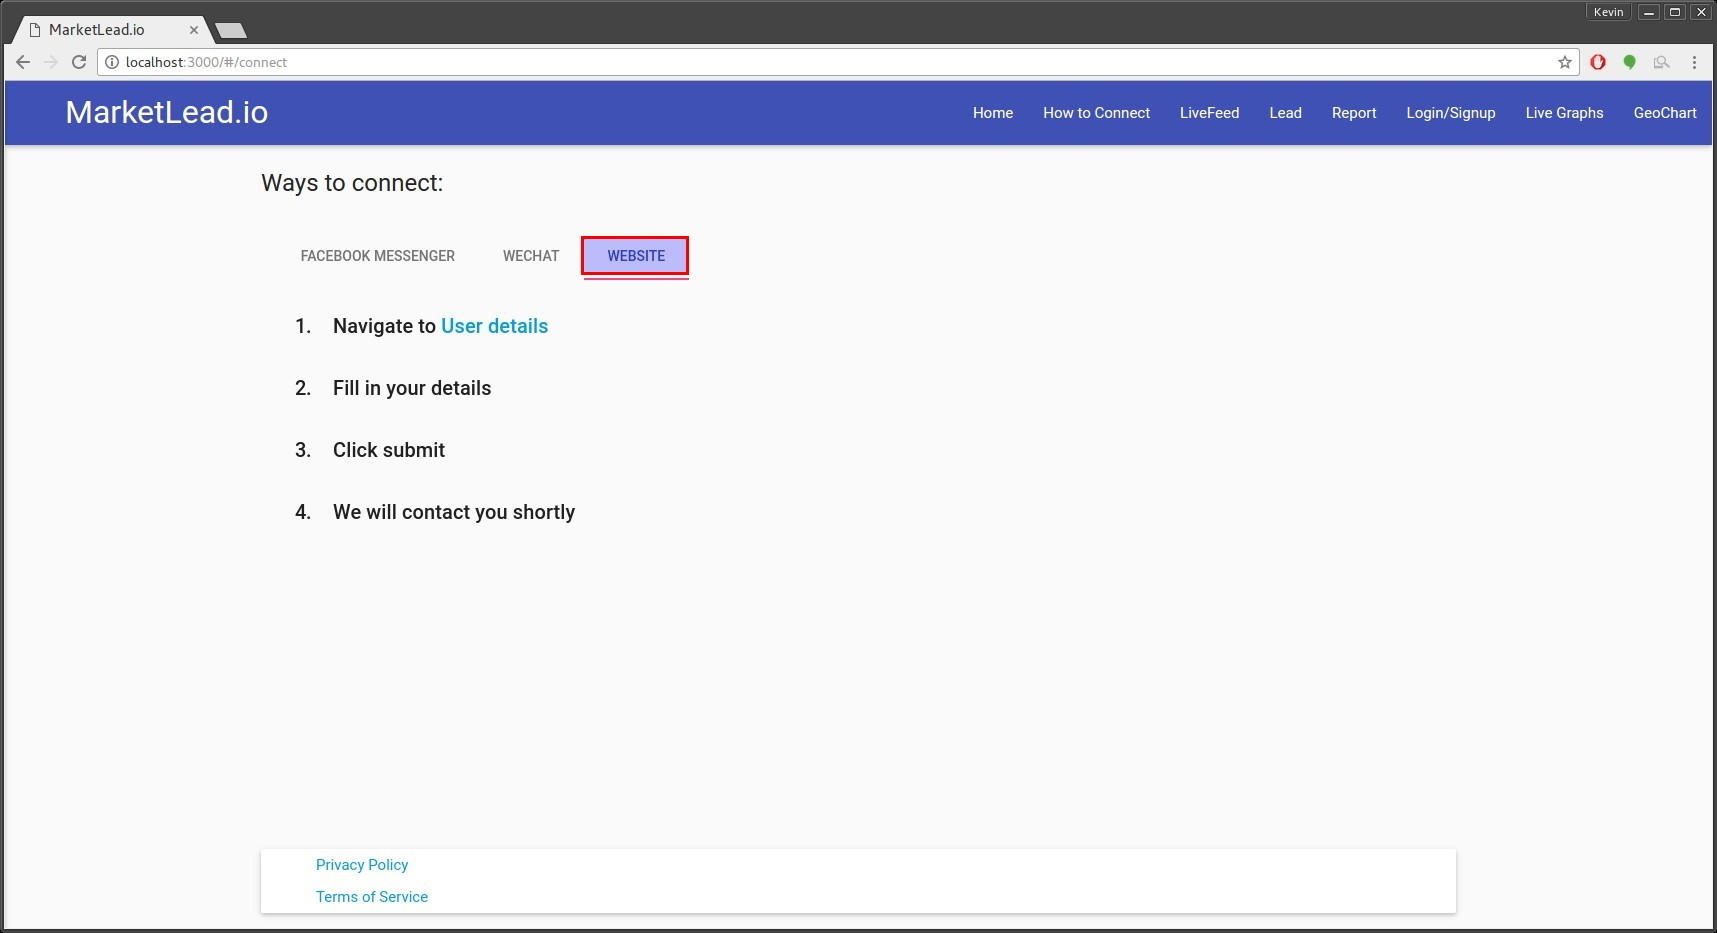
\includegraphics[width=\textwidth]{images/how_to_connect_website.jpg}
					\caption{How to Connect - Website}
					\label{fig:howToConnectWebsite}
				\end{figure}

				\begin{itemize}
					\item Gives a guide to the client on how to fill in a lead without having to use any social media platforms.
					\item This is useful for people that have no social media platforms that connect with our system.
				\end{itemize}

		\subsection{Live Feed}
			\begin{figure}[H]
				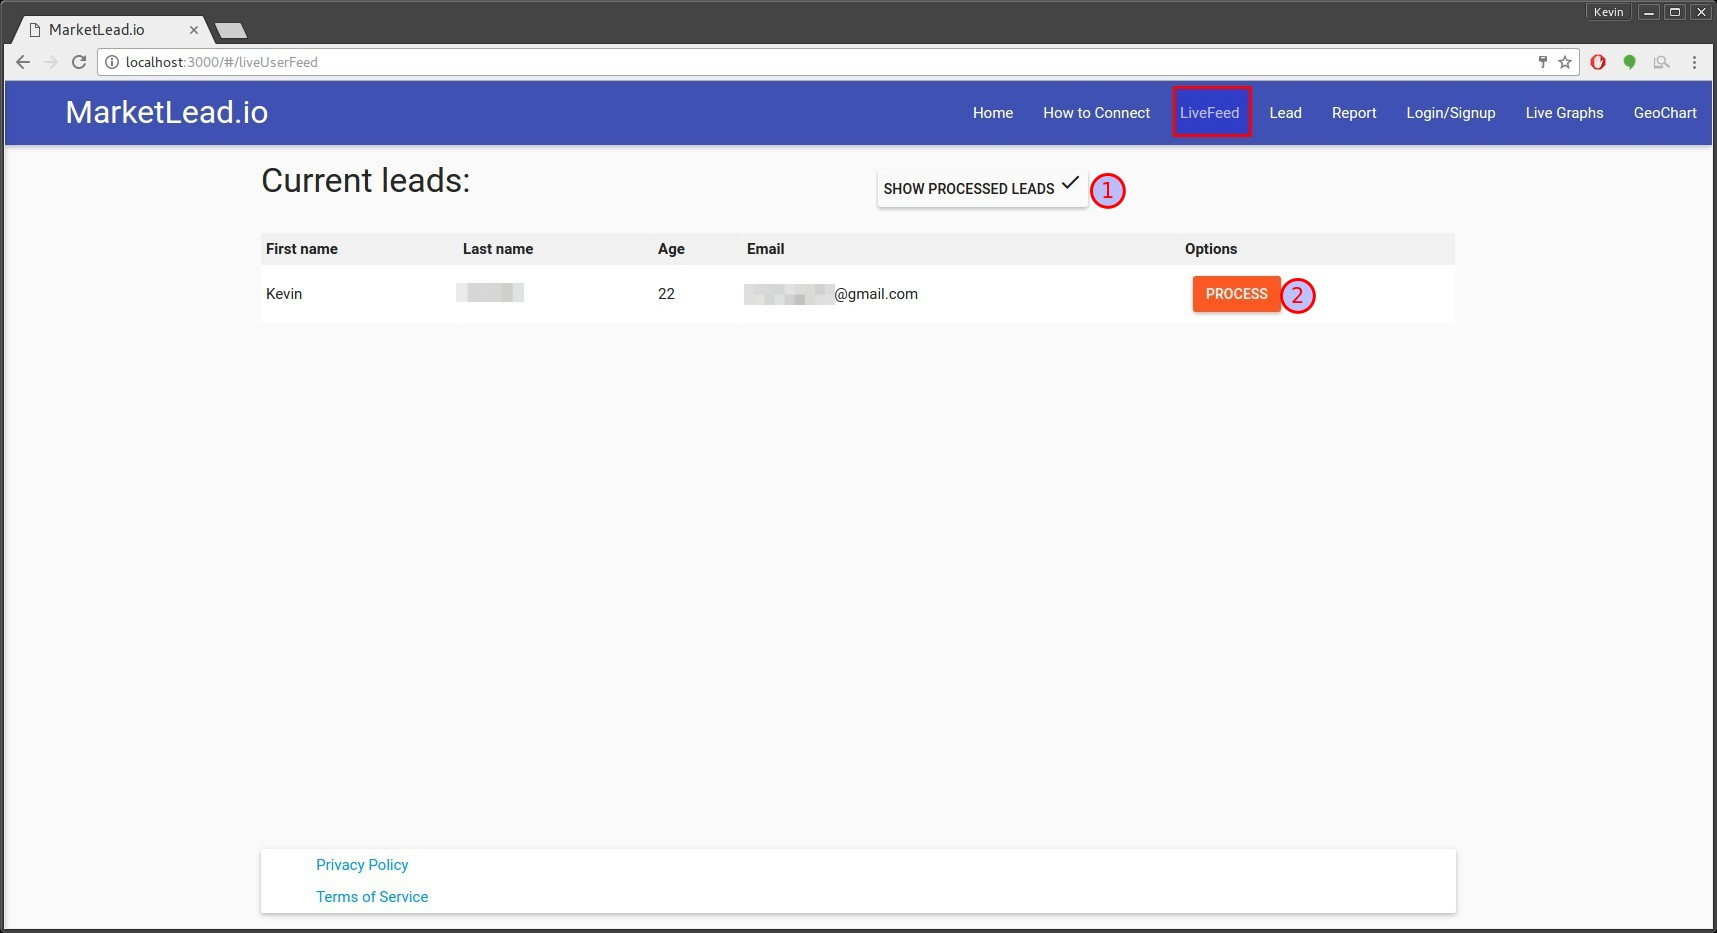
\includegraphics[width=\textwidth]{images/live_feed.jpg}
				\caption{Live Feed}
				\label{fig:liveFeed}
			\end{figure}
			\begin{enumerate}
				\item Will toggle the filter to show data that has/has not been processed yet.
				\item Shows more information about the data record. Once clicked the following will appear.
				\item Before you can view this page you need to be logged in as an analyst or administrator. (If you are not logged in it will take you to log in first)
				\item Shows a live feed of leads and data coming in from the various social media platforms.
				\item This page will automatically load new data as it reaches the system.
				\item This page does not have to be refreshed.
					\begin{figure}[H]
						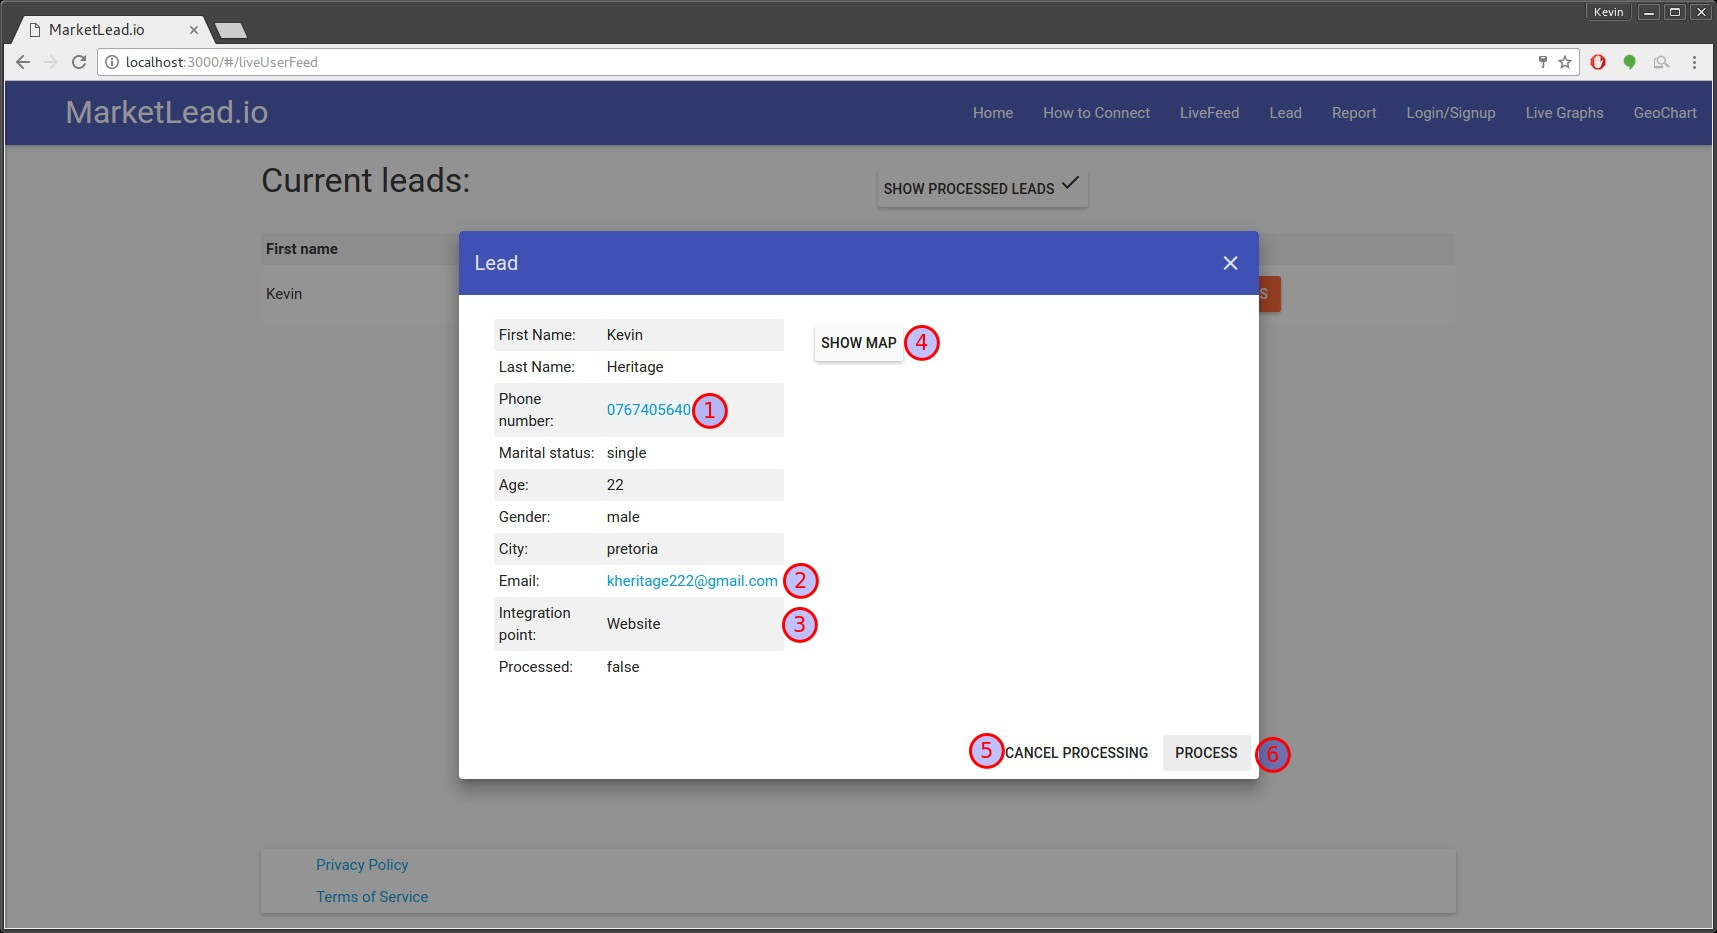
\includegraphics[width=\textwidth]{images/live_feed_process.jpg}
						\caption{Live Feed - Processing of lead}
						\label{fig:liveFeedProcessing}
					\end{figure}

					\begin{itemize}
						\item[1.] When clicked it will open up the application on your computer dealing with phone numbers (Skype). If you are on a mobile device it will open up your phones dialer.
						\item[2.] When clicked it will open your computers default e-mail client. Will also work on mobile.
						\item[3.] Indicates from which point of integration the data came from.
						\item[4.] Will generate a map using the City field to indicate what location the person lives in.
						\item[5.] Clicking this button will not change the "Processed" from false to true but will just close the window.
						\item[6.] Will mark the record as processed and will not be visible in the unprocessed leads filter.
					\end{itemize}
			\end{enumerate}

		\subsection{Lead}
			\begin{figure}[H]
				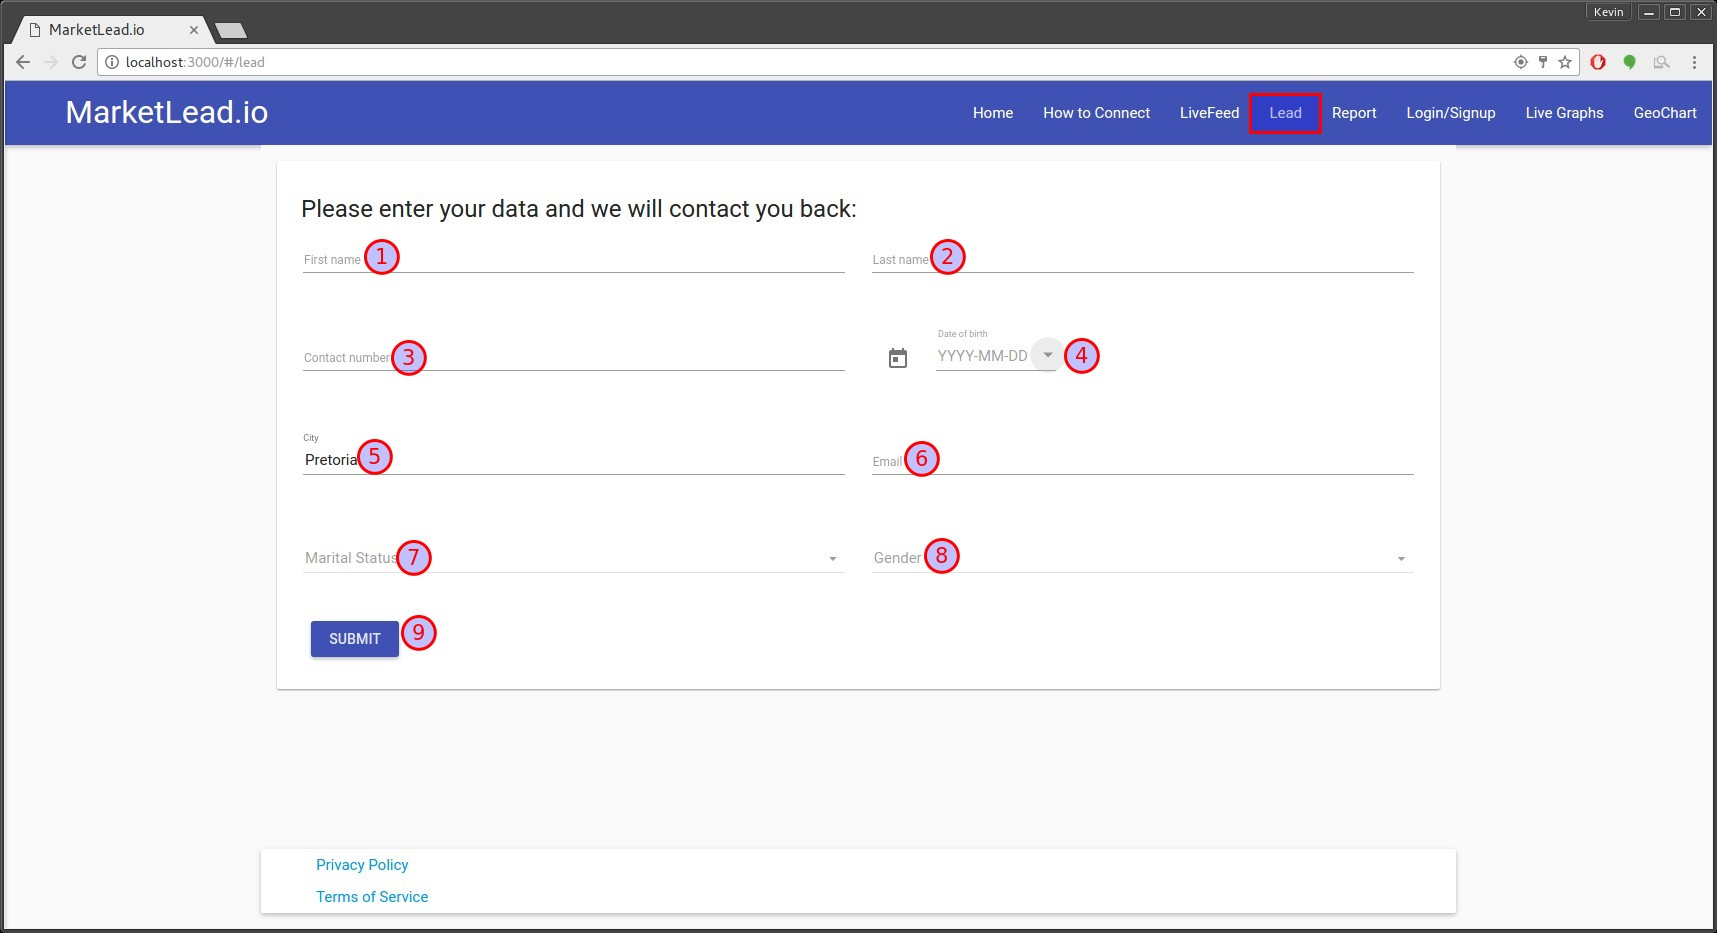
\includegraphics[width=\textwidth]{images/lead.jpg}
				\caption{Lead}
				\label{fig:lead}
			\end{figure}
			Note when loading this page your browser will ask you if you wish to share your location with this site. This will only populate the city field. One can read the privacy policy on our use of your location. We do not save any other information other than the city.
			\begin{enumerate}
				\item Where the user should enter their first names.
				\item Where the user should enter their last name.
				\item Where the user should enter their phone number on which they can be contacted.
				\item Where the user can select their date of birth from the dropdown or enter it manually.
				\item This field should be auto populated if the user allowed the browser to share their location with the website. If the location is incorrect or the user did not share their location they will have to enter the city manually.
				\item Where the user can enter their email address.
				\item Where the user can select their marital status from the pre-populated drop down list.
				\item Where the user can select their gender from the pre-populated drop down list.
				\item Once all of the data has been entered the user can submit their data for processing.
			\end{enumerate}

		\subsection{Report}
			\begin{figure}[H]
				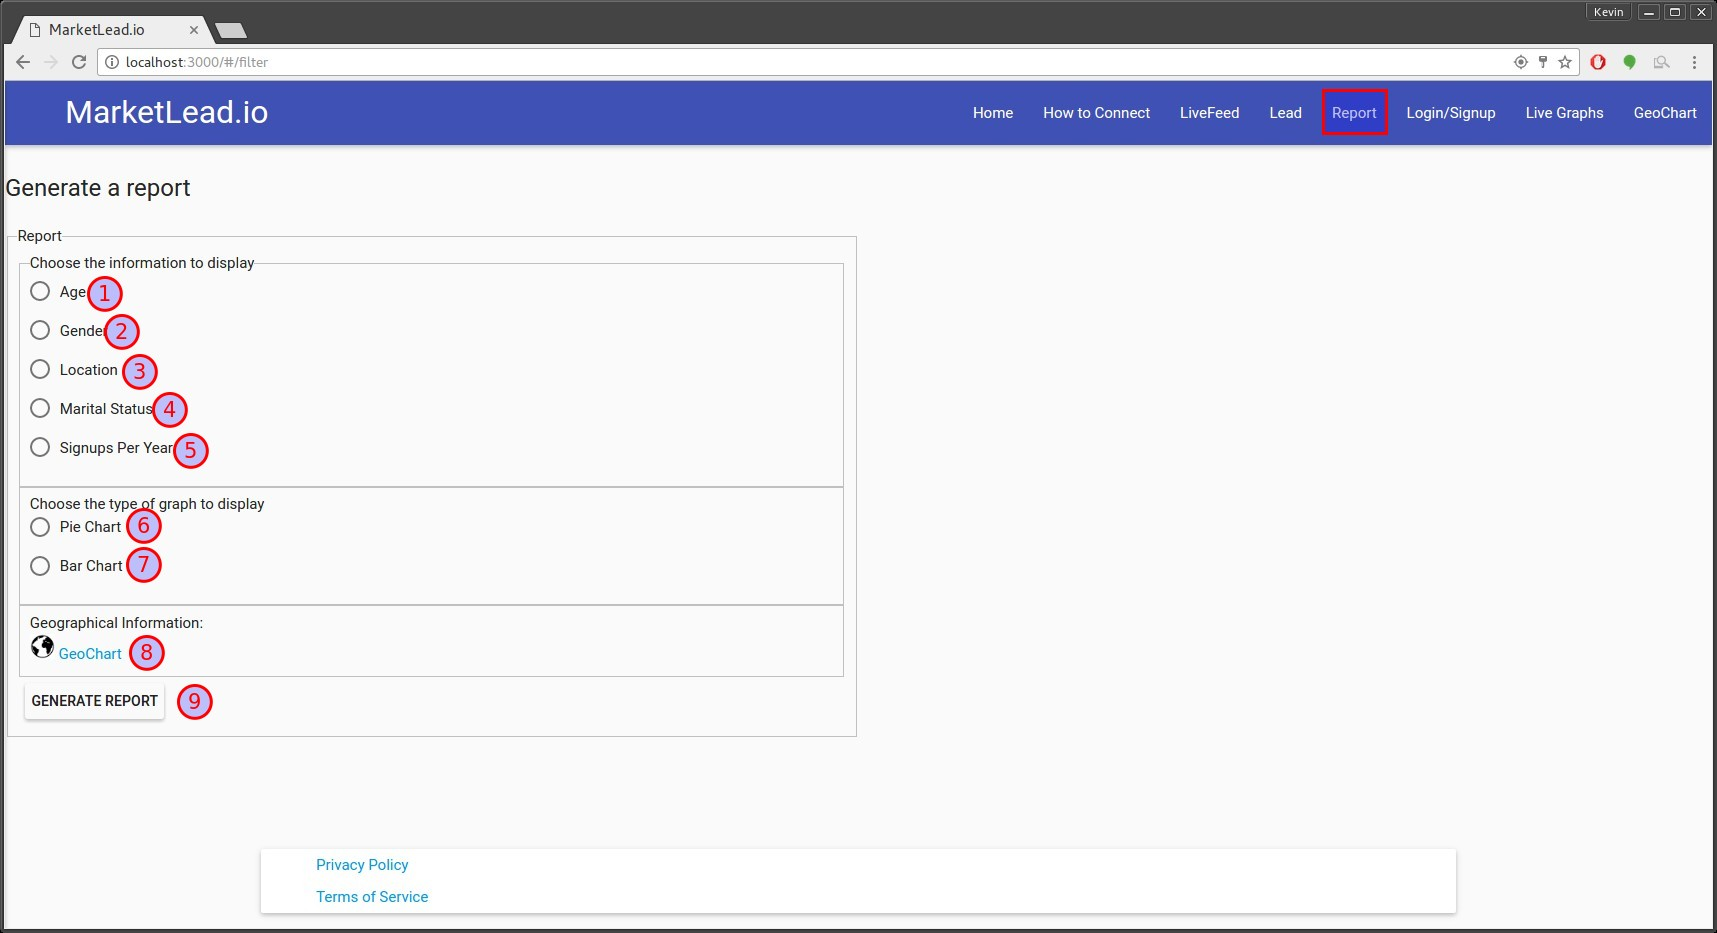
\includegraphics[width=\textwidth]{images/report.jpg}
				\caption{Report}
				\label{fig:report}
			\end{figure}
			Reports of the data can be generated from this page
			\begin{enumerate}
				\item Filters the report by clients age.
				\item Filters the data by clients gender.
				\item Filter the data by clients location.
				\item Filters the data by clients marital status.
				\item Filters the data by signups per year.
				\item Specifies that a pie chart needs to be generated.
				\item Specifies that a bar chart needs to be generated.
				\item Specifies that a Geographical Chart needs to be generated.\\
					Note: This option will not take any other fields and will generate a map with the number of clients from each city.
				\item Generates the report based on the above data that was selected.
			\end{enumerate}

		\subsection{Login/Signup}
			\begin{figure}[H]
				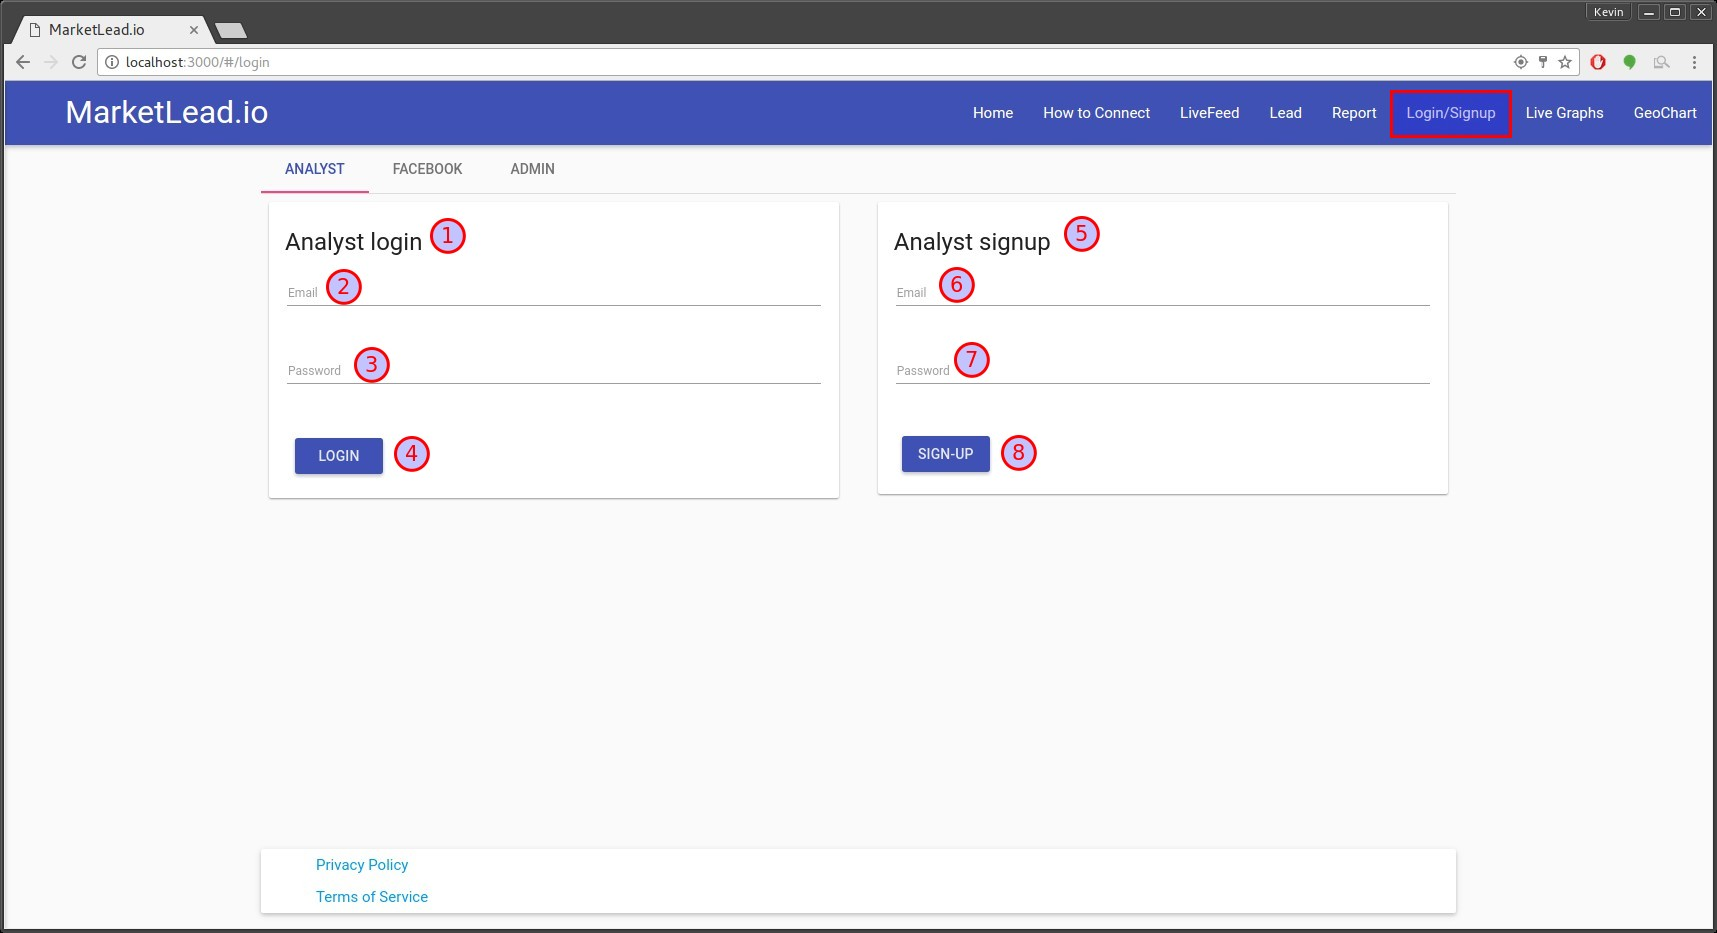
\includegraphics[width=\textwidth]{images/login_signup.jpg}
				\caption{Login/Signup - Analyst}
				\label{fig:loginSignupAnalyst}
			\end{figure}
			This is the page that will initially be loaded when navigating to the Login/Signup page
			
			\subsubsection{Analyst}
				\begin{enumerate}
					\item Section for analyst to login if they already have an account on the website.
					\item Where the analyst should enter their email that is registered on the system.
					\item Where the analyst should enter their password associated with the email they entered.
					\item Button to log them in for this session.
					\item Section for analysts to sign up to use the system.
					\item The email address they wish to sign up with.
					\item The password they wish to associate with their email address to sign up.
					\item Button to sign up the analyst. The analyst should then log in to the system following steps 1-4.
				\end{enumerate}

			\subsubsection{Facebook}
				\begin{figure}[H]
					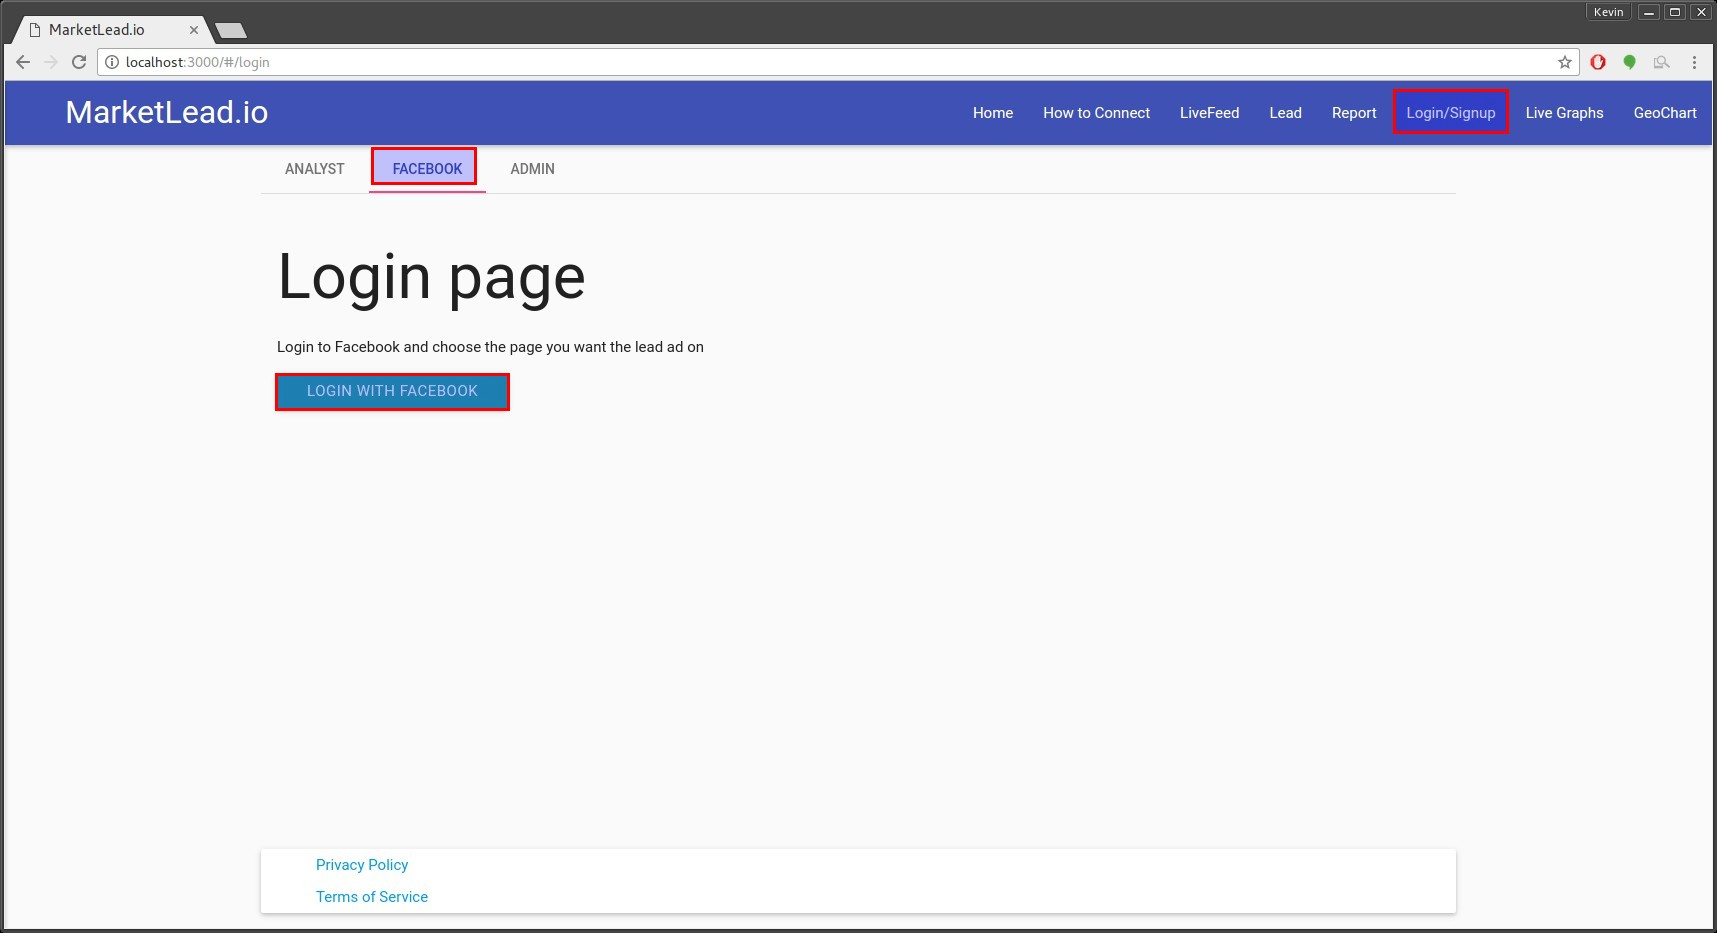
\includegraphics[width=\textwidth]{images/login_signup_facebook.jpg}
					\caption{Login/Signup - Facebook}
					\label{fig:loginSignupFacebook}
				\end{figure}
				This is specifically for when a marketer wants to link their Facebook page to send the lead ad data through to our system for processing.
				Once the login button is clicked facebook will load and let you log in.

				\begin{figure}[H]
					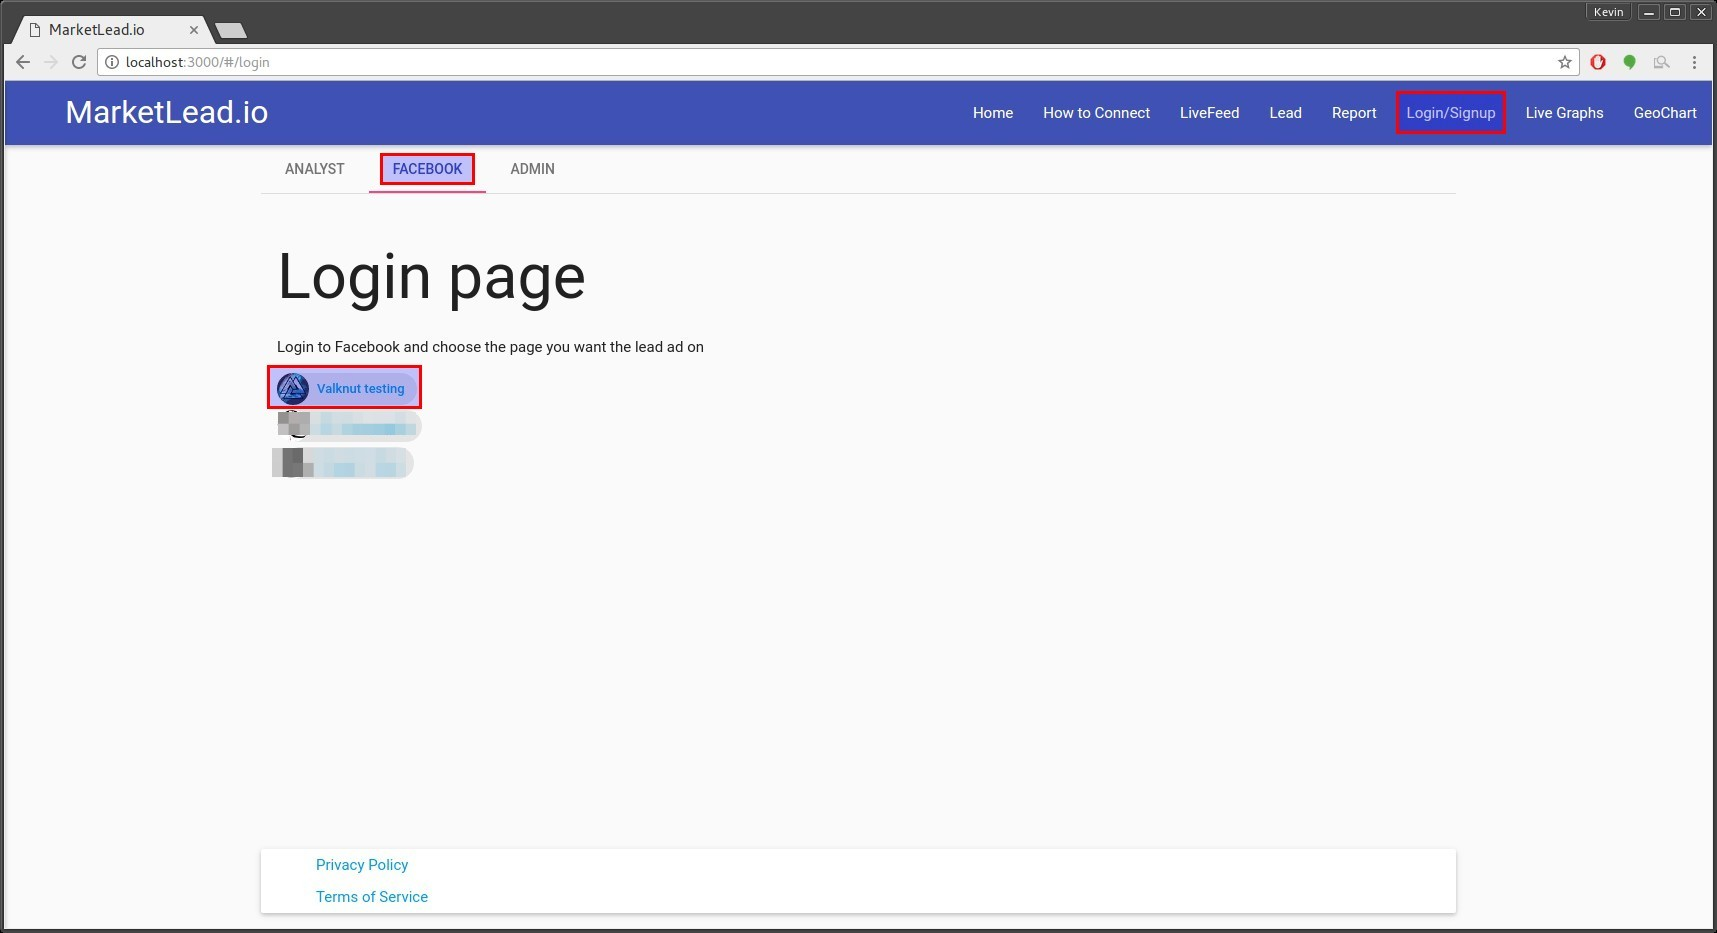
\includegraphics[width=\textwidth]{images/login_signup_facebook_pages.jpg}
					\caption{Login/Signup - Facebook Pages}
					\label{fig:loginSignupFacebookPages}
				\end{figure}
				Once logged in the page will load your pages. Select the page you wish to interact with our system.
				Once this page has been clicked it will send all of its data gathered from Lead Ads to our system for processing.

		\subsection{Live Graphs}
			\begin{figure}[H]
				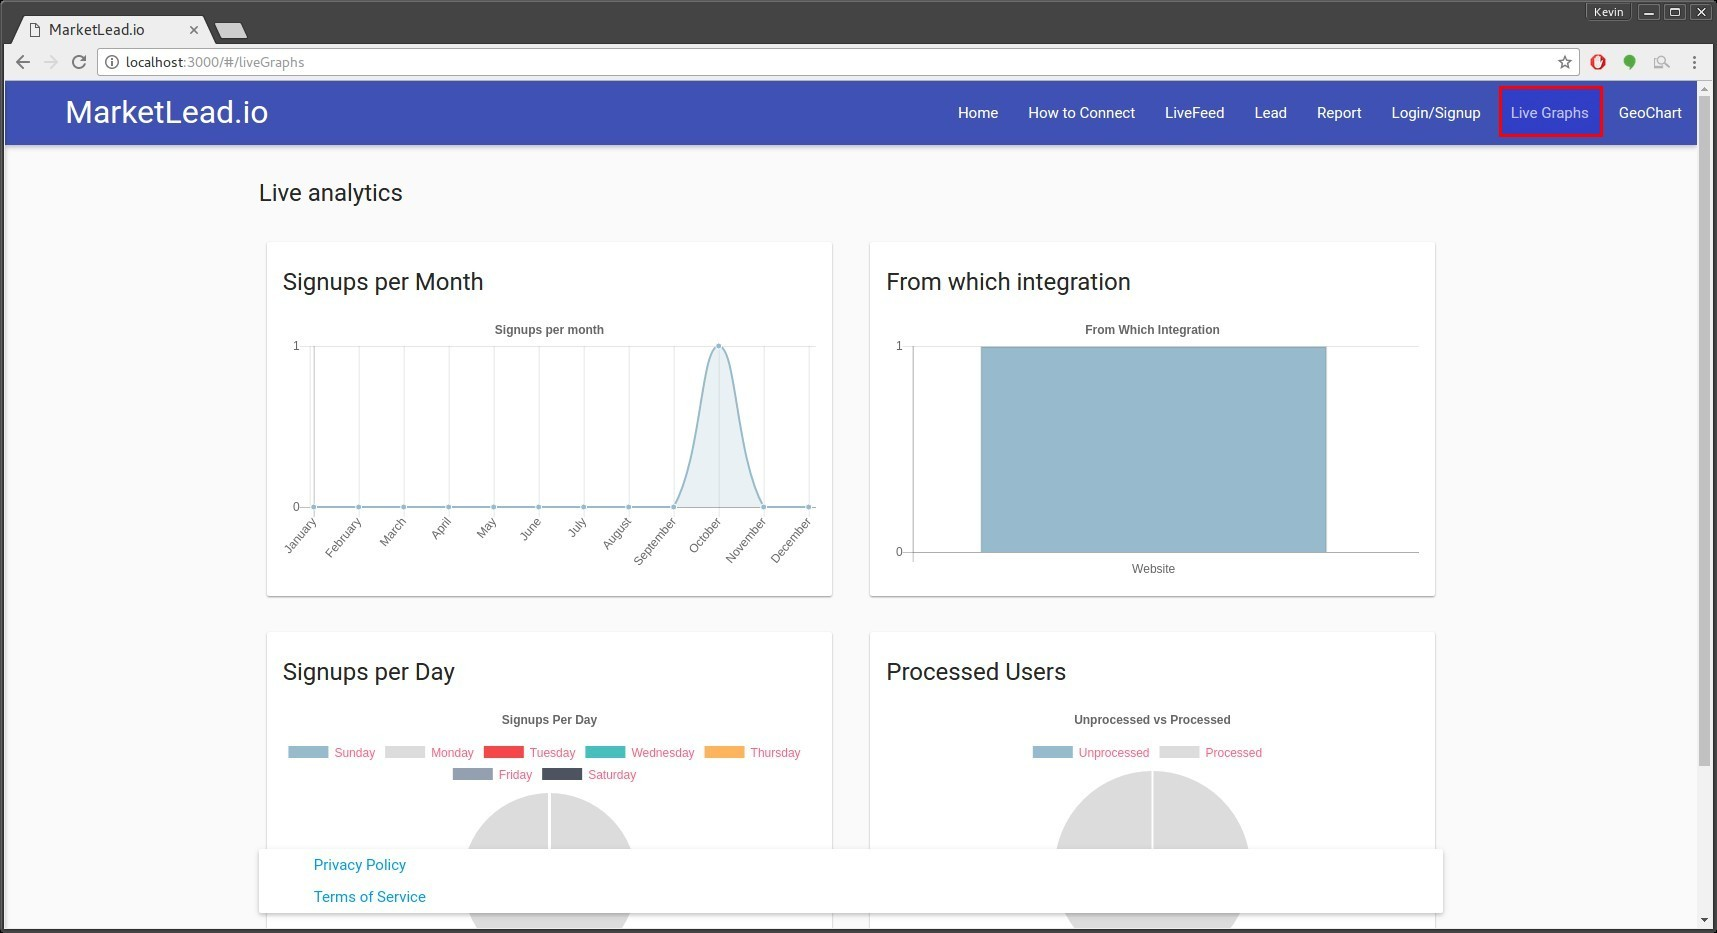
\includegraphics[width=\textwidth]{images/live_graph.jpg}
				\caption{Live Graphs}
				\label{fig:liveGraphs}
			\end{figure}

			\begin{itemize}
				\item All of these graphs will update as data is caught by the server. (No need to refresh this page)
				\item Hovering over any of these graphs will give you some more information about the section you are hovering over.
			\end{itemize}

		\subsection{GeoChart}
			\begin{figure}[H]
				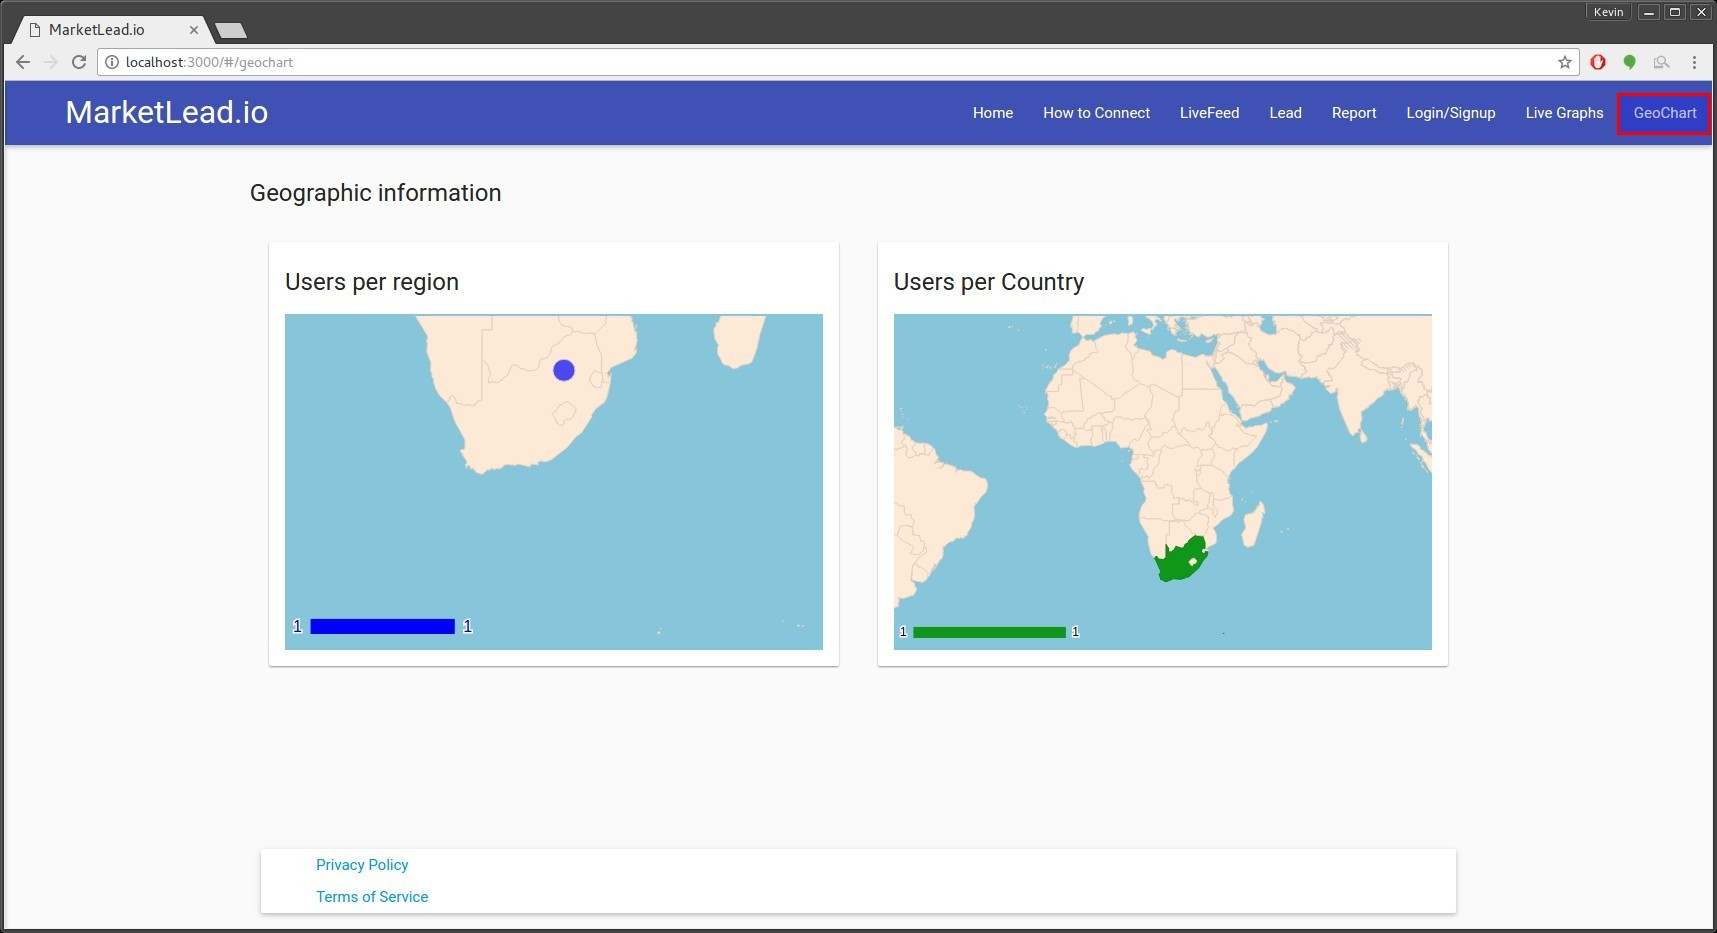
\includegraphics[width=\textwidth]{images/geo_chart.jpg}
				\caption{GeoChart}
				\label{fig:geoChart}
			\end{figure}

			\begin{itemize}
				\item These graphs will also update in real time as data is caught by the system. (No need to refresh)
				\item Hovering over sections of these graphs will also provide more information about the section you are hovering over.
			\end{itemize}

	\section{Trouble Shooting}
		The steps below each problem is steps you can try to get the system working.
		One does not have to follow each step but can start from the top until the problem is resolved.
		\begin{itemize}
			\item If some component of the web interface stops working
				\begin{enumerate}
					\item Press F5 on your keyboard to refresh the web page.
					\item Check your internet connection.
					\item Be patient if you have a slow internet connection.
				\end{enumerate}
			\item If you cannot access a part of the web interface
				\begin{enumerate}
					\item Make sure you are logged in.
					\item Make sure that you are logged into the account with the appropriate permissions.
				\end{enumerate}
			\item If you cannot access the web interface at all
				\begin{enumerate}
					\item Make sure you are connected to the internet.
					\item Refresh the page a few times.
				\end{enumerate}
		\end{itemize}

	\section{References to other documentation}
		\begin{itemize}
			\item{Requirements specifications as per 12 October 2016}
			\item{Architecture Design as per 12 October 2016}
			\item{\href{https://www.facebook.com/business/a/lead-ads}{Facebook Lead adverts} as per 12 October 2016}
		\end{itemize}

\end{document}
